\documentclass[11pt,compress,t,notes=noshow, xcolor=table]{beamer}
\usepackage[]{graphicx}\usepackage[]{color}
% maxwidth is the original width if it is less than linewidth
% otherwise use linewidth (to make sure the graphics do not exceed the margin)
\makeatletter
\def\maxwidth{ %
  \ifdim\Gin@nat@width>\linewidth
    \linewidth
  \else
    \Gin@nat@width
  \fi
}
\makeatother

\definecolor{fgcolor}{rgb}{0.345, 0.345, 0.345}
\newcommand{\hlnum}[1]{\textcolor[rgb]{0.686,0.059,0.569}{#1}}%
\newcommand{\hlstr}[1]{\textcolor[rgb]{0.192,0.494,0.8}{#1}}%
\newcommand{\hlcom}[1]{\textcolor[rgb]{0.678,0.584,0.686}{\textit{#1}}}%
\newcommand{\hlopt}[1]{\textcolor[rgb]{0,0,0}{#1}}%
\newcommand{\hlstd}[1]{\textcolor[rgb]{0.345,0.345,0.345}{#1}}%
\newcommand{\hlkwa}[1]{\textcolor[rgb]{0.161,0.373,0.58}{\textbf{#1}}}%
\newcommand{\hlkwb}[1]{\textcolor[rgb]{0.69,0.353,0.396}{#1}}%
\newcommand{\hlkwc}[1]{\textcolor[rgb]{0.333,0.667,0.333}{#1}}%
\newcommand{\hlkwd}[1]{\textcolor[rgb]{0.737,0.353,0.396}{\textbf{#1}}}%
\let\hlipl\hlkwb

\usepackage{framed}
\makeatletter
\newenvironment{kframe}{%
 \def\at@end@of@kframe{}%
 \ifinner\ifhmode%
  \def\at@end@of@kframe{\end{minipage}}%
  \begin{minipage}{\columnwidth}%
 \fi\fi%
 \def\FrameCommand##1{\hskip\@totalleftmargin \hskip-\fboxsep
 \colorbox{shadecolor}{##1}\hskip-\fboxsep
     % There is no \\@totalrightmargin, so:
     \hskip-\linewidth \hskip-\@totalleftmargin \hskip\columnwidth}%
 \MakeFramed {\advance\hsize-\width
   \@totalleftmargin\z@ \linewidth\hsize
   \@setminipage}}%
 {\par\unskip\endMakeFramed%
 \at@end@of@kframe}
\makeatother

\definecolor{shadecolor}{rgb}{.97, .97, .97}
\definecolor{messagecolor}{rgb}{0, 0, 0}
\definecolor{warningcolor}{rgb}{1, 0, 1}
\definecolor{errorcolor}{rgb}{1, 0, 0}
\newenvironment{knitrout}{}{} % an empty environment to be redefined in TeX

\usepackage{alltt}
\newcommand{\SweaveOpts}[1]{}  % do not interfere with LaTeX
\newcommand{\SweaveInput}[1]{} % because they are not real TeX commands
\newcommand{\Sexpr}[1]{}       % will only be parsed by R
\newcommand{\xmark}{\ding{55}}%


\usepackage[english]{babel}
\usepackage[utf8]{inputenc}

\usepackage{dsfont}
\usepackage{verbatim}
\usepackage{amsmath}
\usepackage{amsfonts}
\usepackage{amssymb}
\usepackage{bm}
\usepackage{csquotes}
\usepackage{multirow}
\usepackage{longtable}
\usepackage{booktabs}
\usepackage{enumerate}
\usepackage[absolute,overlay]{textpos}
\usepackage{psfrag}
\usepackage{algorithm}
\usepackage{algpseudocode}
\usepackage{eqnarray}
\usepackage{arydshln}
\usepackage{tabularx}
\usepackage{placeins}
\usepackage{tikz}
\usepackage{setspace}
\usepackage{colortbl}
\usepackage{mathtools}
\usepackage{wrapfig}
\usepackage{bm}
\usepackage{amsmath}
\usepackage{pifont}
\usepackage[round]{natbib}
\usepackage{hyperref}

\usetikzlibrary{shapes,arrows,automata,positioning,calc,chains,trees, shadows}
\tikzset{
  %Define standard arrow tip
  >=stealth',
  %Define style for boxes
  punkt/.style={
    rectangle,
    rounded corners,
    draw=black, very thick,
    text width=6.5em,
    minimum height=2em,
    text centered},
  % Define arrow style
  pil/.style={
    ->,
    thick,
    shorten <=2pt,
    shorten >=2pt,}
}

\usepackage{subfig}

% Defines macros and environments
\usepackage{../../style/lmu-lecture}


\let\code=\texttt
\let\proglang=\textsf

\setkeys{Gin}{width=0.9\textwidth}

\setbeamertemplate{frametitle}{\expandafter\uppercase\expandafter\insertframetitle}

% basic latex stuff
\newcommand{\pkg}[1]{{\fontseries{b}\selectfont #1}} % fontstyle for R packages

% Often used in exercise Rnw files, still relevant?
\newcommand{\lz}{\vspace{0.5cm}} % vertical space
\newcommand{\dlz}{\vspace{1cm}}  % double vertical space

% Unused and about to be deleted
\newcommand{\oneliner}[1] % Oneliner for important statements
{\begin{block}{}\begin{center}\begin{Large}#1\end{Large}\end{center}\end{block}}


%--------------------%
%  New environments  %
%--------------------%

 % Frame with breaks and verbatim // this is used very often
\newenvironment{vbframe}
{
\begin{frame}[containsverbatim,allowframebreaks]
}
{
\end{frame}
}

% Frame with verbatim without breaks (to avoid numbering one slided frames)
% This is not used anywhere but I can see it being useful
\newenvironment{vframe}
{
\begin{frame}[containsverbatim]
}
{
\end{frame}
}

% Itemize block
\newenvironment{blocki}[1]
{
\begin{block}{#1}\begin{itemize}
}
{
\end{itemize}\end{block}
}

%--------------%
%  Citebutton  %
%--------------%
% Example usage (from slides-cart-discussion.tex)
% \citebutton{Breiman, 1984}{https://www.taylorfrancis.com/books/mono/10.1201/9781315139470/classification-regression-trees-leo-breiman}
\newcommand{\citebutton}[2]{%
\NoCaseChange{\resizebox{!}{9pt}{\protect\beamergotobutton{\href{#2}{#1}}}}%
}

% textcolor that works in mathmode
% https://tex.stackexchange.com/a/261480
% Used e.g. in forests/slides-forests-bagging.tex
% [...] \textcolor{blue}{\tfrac{1}{M}\sum^M_{m} [...]
\makeatletter
\renewcommand*{\@textcolor}[3]{%
  \protect\leavevmode
  \begingroup
    \color#1{#2}#3%
  \endgroup
}
\makeatother




 
% dependencies: amsmath, amssymb, dsfont
% math spaces
\ifdefined\N
\renewcommand{\N}{\mathds{N}} % N, naturals
\else \newcommand{\N}{\mathds{N}} \fi
\newcommand{\Z}{\mathds{Z}} % Z, integers
\newcommand{\Q}{\mathds{Q}} % Q, rationals
\newcommand{\R}{\mathds{R}} % R, reals
\ifdefined\C
\renewcommand{\C}{\mathds{C}} % C, complex
\else \newcommand{\C}{\mathds{C}} \fi
\newcommand{\continuous}{\mathcal{C}} % C, space of continuous functions
\newcommand{\M}{\mathcal{M}} % machine numbers
\newcommand{\epsm}{\epsilon_m} % maximum error

% counting / finite sets
\newcommand{\setzo}{\{0, 1\}} % set 0, 1
\newcommand{\setmp}{\{-1, +1\}} % set -1, 1
\newcommand{\unitint}{[0, 1]} % unit interval

% basic math stuff
\newcommand{\xt}{\tilde x} % x tilde
\DeclareMathOperator*{\argmax}{arg\,max} % argmax
\DeclareMathOperator*{\argmin}{arg\,min} % argmin
\newcommand{\argminlim}{\mathop{\mathrm{arg\,min}}\limits} % argmax with limits
\newcommand{\argmaxlim}{\mathop{\mathrm{arg\,max}}\limits} % argmin with limits
\newcommand{\sign}{\operatorname{sign}} % sign, signum
\newcommand{\I}{\mathbb{I}} % I, indicator
\newcommand{\order}{\mathcal{O}} % O, order
\newcommand{\bigO}{\mathcal{O}} % Big-O Landau
\newcommand{\littleo}{{o}} % Little-o Landau
\newcommand{\pd}[2]{\frac{\partial{#1}}{\partial #2}} % partial derivative
\newcommand{\floorlr}[1]{\left\lfloor #1 \right\rfloor} % floor
\newcommand{\ceillr}[1]{\left\lceil #1 \right\rceil} % ceiling
\newcommand{\indep}{\perp \!\!\! \perp} % independence symbol

% sums and products
\newcommand{\sumin}{\sum\limits_{i=1}^n} % summation from i=1 to n
\newcommand{\sumim}{\sum\limits_{i=1}^m} % summation from i=1 to m
\newcommand{\sumjn}{\sum\limits_{j=1}^n} % summation from j=1 to p
\newcommand{\sumjp}{\sum\limits_{j=1}^p} % summation from j=1 to p
\newcommand{\sumik}{\sum\limits_{i=1}^k} % summation from i=1 to k
\newcommand{\sumkg}{\sum\limits_{k=1}^g} % summation from k=1 to g
\newcommand{\sumjg}{\sum\limits_{j=1}^g} % summation from j=1 to g
\newcommand{\meanin}{\frac{1}{n} \sum\limits_{i=1}^n} % mean from i=1 to n
\newcommand{\meanim}{\frac{1}{m} \sum\limits_{i=1}^m} % mean from i=1 to n
\newcommand{\meankg}{\frac{1}{g} \sum\limits_{k=1}^g} % mean from k=1 to g
\newcommand{\prodin}{\prod\limits_{i=1}^n} % product from i=1 to n
\newcommand{\prodkg}{\prod\limits_{k=1}^g} % product from k=1 to g
\newcommand{\prodjp}{\prod\limits_{j=1}^p} % product from j=1 to p

% linear algebra
\newcommand{\one}{\bm{1}} % 1, unitvector
\newcommand{\zero}{\mathbf{0}} % 0-vector
\newcommand{\id}{\bm{I}} % I, identity
\newcommand{\diag}{\operatorname{diag}} % diag, diagonal
\newcommand{\trace}{\operatorname{tr}} % tr, trace
\newcommand{\spn}{\operatorname{span}} % span
\newcommand{\scp}[2]{\left\langle #1, #2 \right\rangle} % <.,.>, scalarproduct
\newcommand{\mat}[1]{\begin{pmatrix} #1 \end{pmatrix}} % short pmatrix command
\newcommand{\Amat}{\mathbf{A}} % matrix A
\newcommand{\Deltab}{\mathbf{\Delta}} % error term for vectors

% basic probability + stats
\renewcommand{\P}{\mathds{P}} % P, probability
\newcommand{\E}{\mathds{E}} % E, expectation
\newcommand{\var}{\mathsf{Var}} % Var, variance
\newcommand{\cov}{\mathsf{Cov}} % Cov, covariance
\newcommand{\corr}{\mathsf{Corr}} % Corr, correlation
\newcommand{\normal}{\mathcal{N}} % N of the normal distribution
\newcommand{\iid}{\overset{i.i.d}{\sim}} % dist with i.i.d superscript
\newcommand{\distas}[1]{\overset{#1}{\sim}} % ... is distributed as ...

% machine learning
\newcommand{\Xspace}{\mathcal{X}} % X, input space
\newcommand{\Yspace}{\mathcal{Y}} % Y, output space
\newcommand{\Zspace}{\mathcal{Z}} % Z, space of sampled datapoints
\newcommand{\nset}{\{1, \ldots, n\}} % set from 1 to n
\newcommand{\pset}{\{1, \ldots, p\}} % set from 1 to p
\newcommand{\gset}{\{1, \ldots, g\}} % set from 1 to g
\newcommand{\Pxy}{\mathbb{P}_{xy}} % P_xy
\newcommand{\Exy}{\mathbb{E}_{xy}} % E_xy: Expectation over random variables xy
\newcommand{\xv}{\mathbf{x}} % vector x (bold)
\newcommand{\xtil}{\tilde{\mathbf{x}}} % vector x-tilde (bold)
\newcommand{\yv}{\mathbf{y}} % vector y (bold)
\newcommand{\xy}{(\xv, y)} % observation (x, y)
\newcommand{\xvec}{\left(x_1, \ldots, x_p\right)^\top} % (x1, ..., xp)
\newcommand{\Xmat}{\mathbf{X}} % Design matrix
\newcommand{\allDatasets}{\mathds{D}} % The set of all datasets
\newcommand{\allDatasetsn}{\mathds{D}_n}  % The set of all datasets of size n
\newcommand{\D}{\mathcal{D}} % D, data
\newcommand{\Dn}{\D_n} % D_n, data of size n
\newcommand{\Dtrain}{\mathcal{D}_{\text{train}}} % D_train, training set
\newcommand{\Dtest}{\mathcal{D}_{\text{test}}} % D_test, test set
\newcommand{\xyi}[1][i]{\left(\xv^{(#1)}, y^{(#1)}\right)} % (x^i, y^i), i-th observation
\newcommand{\Dset}{\left( \xyi[1], \ldots, \xyi[n]\right)} % {(x1,y1)), ..., (xn,yn)}, data
\newcommand{\defAllDatasetsn}{(\Xspace \times \Yspace)^n} % Def. of the set of all datasets of size n
\newcommand{\defAllDatasets}{\bigcup_{n \in \N}(\Xspace \times \Yspace)^n} % Def. of the set of all datasets
\newcommand{\xdat}{\left\{ \xv^{(1)}, \ldots, \xv^{(n)}\right\}} % {x1, ..., xn}, input data
\newcommand{\ydat}{\left\{ \yv^{(1)}, \ldots, \yv^{(n)}\right\}} % {y1, ..., yn}, input data
\newcommand{\yvec}{\left(y^{(1)}, \hdots, y^{(n)}\right)^\top} % (y1, ..., yn), vector of outcomes
\newcommand{\greekxi}{\xi} % Greek letter xi
\renewcommand{\xi}[1][i]{\xv^{(#1)}} % x^i, i-th observed value of x
\newcommand{\yi}[1][i]{y^{(#1)}} % y^i, i-th observed value of y
\newcommand{\xivec}{\left(x^{(i)}_1, \ldots, x^{(i)}_p\right)^\top} % (x1^i, ..., xp^i), i-th observation vector
\newcommand{\xj}{\xv_j} % x_j, j-th feature
\newcommand{\xjvec}{\left(x^{(1)}_j, \ldots, x^{(n)}_j\right)^\top} % (x^1_j, ..., x^n_j), j-th feature vector
\newcommand{\phiv}{\mathbf{\phi}} % Basis transformation function phi
\newcommand{\phixi}{\mathbf{\phi}^{(i)}} % Basis transformation of xi: phi^i := phi(xi)

%%%%%% ml - models general
\newcommand{\lamv}{\bm{\lambda}} % lambda vector, hyperconfiguration vector
\newcommand{\Lam}{\bm{\Lambda}}	 % Lambda, space of all hpos
% Inducer / Inducing algorithm
\newcommand{\preimageInducer}{\left(\defAllDatasets\right)\times\Lam} % Set of all datasets times the hyperparameter space
\newcommand{\preimageInducerShort}{\allDatasets\times\Lam} % Set of all datasets times the hyperparameter space
% Inducer / Inducing algorithm
\newcommand{\ind}{\mathcal{I}} % Inducer, inducing algorithm, learning algorithm

% continuous prediction function f
\newcommand{\ftrue}{f_{\text{true}}}  % True underlying function (if a statistical model is assumed)
\newcommand{\ftruex}{\ftrue(\xv)} % True underlying function (if a statistical model is assumed)
\newcommand{\fx}{f(\xv)} % f(x), continuous prediction function
\newcommand{\fdomains}{f: \Xspace \rightarrow \R^g} % f with domain and co-domain
\newcommand{\Hspace}{\mathcal{H}} % hypothesis space where f is from
\newcommand{\fbayes}{f^{\ast}} % Bayes-optimal model
\newcommand{\fxbayes}{f^{\ast}(\xv)} % Bayes-optimal model
\newcommand{\fkx}[1][k]{f_{#1}(\xv)} % f_j(x), discriminant component function
\newcommand{\fh}{\hat{f}} % f hat, estimated prediction function
\newcommand{\fxh}{\fh(\xv)} % fhat(x)
\newcommand{\fxt}{f(\xv ~|~ \thetav)} % f(x | theta)
\newcommand{\fxi}{f\left(\xv^{(i)}\right)} % f(x^(i))
\newcommand{\fxih}{\hat{f}\left(\xv^{(i)}\right)} % f(x^(i))
\newcommand{\fxit}{f\left(\xv^{(i)} ~|~ \thetav\right)} % f(x^(i) | theta)
\newcommand{\fhD}{\fh_{\D}} % fhat_D, estimate of f based on D
\newcommand{\fhDtrain}{\fh_{\Dtrain}} % fhat_Dtrain, estimate of f based on D
\newcommand{\fhDnlam}{\fh_{\Dn, \lamv}} %model learned on Dn with hp lambda
\newcommand{\fhDlam}{\fh_{\D, \lamv}} %model learned on D with hp lambda
\newcommand{\fhDnlams}{\fh_{\Dn, \lamv^\ast}} %model learned on Dn with optimal hp lambda
\newcommand{\fhDlams}{\fh_{\D, \lamv^\ast}} %model learned on D with optimal hp lambda

% discrete prediction function h
\newcommand{\hx}{h(\xv)} % h(x), discrete prediction function
\newcommand{\hh}{\hat{h}} % h hat
\newcommand{\hxh}{\hat{h}(\xv)} % hhat(x)
\newcommand{\hxt}{h(\xv | \thetav)} % h(x | theta)
\newcommand{\hxi}{h\left(\xi\right)} % h(x^(i))
\newcommand{\hxit}{h\left(\xi ~|~ \thetav\right)} % h(x^(i) | theta)
\newcommand{\hbayes}{h^{\ast}} % Bayes-optimal classification model
\newcommand{\hxbayes}{h^{\ast}(\xv)} % Bayes-optimal classification model

% yhat
\newcommand{\yh}{\hat{y}} % yhat for prediction of target
\newcommand{\yih}{\hat{y}^{(i)}} % yhat^(i) for prediction of ith targiet
\newcommand{\resi}{\yi- \yih}

% theta
\newcommand{\thetah}{\hat{\theta}} % theta hat
\newcommand{\thetav}{\bm{\theta}} % theta vector
\newcommand{\thetavh}{\bm{\hat\theta}} % theta vector hat
\newcommand{\thetat}[1][t]{\thetav^{[#1]}} % theta^[t] in optimization
\newcommand{\thetatn}[1][t]{\thetav^{[#1 +1]}} % theta^[t+1] in optimization
\newcommand{\thetahDnlam}{\thetavh_{\Dn, \lamv}} %theta learned on Dn with hp lambda
\newcommand{\thetahDlam}{\thetavh_{\D, \lamv}} %theta learned on D with hp lambda
\newcommand{\mint}{\min_{\thetav \in \Theta}} % min problem theta
\newcommand{\argmint}{\argmin_{\thetav \in \Theta}} % argmin theta

% densities + probabilities
% pdf of x
\newcommand{\pdf}{p} % p
\newcommand{\pdfx}{p(\xv)} % p(x)
\newcommand{\pixt}{\pi(\xv~|~ \thetav)} % pi(x|theta), pdf of x given theta
\newcommand{\pixit}[1][i]{\pi\left(\xi[#1] ~|~ \thetav\right)} % pi(x^i|theta), pdf of x given theta
\newcommand{\pixii}[1][i]{\pi\left(\xi[#1]\right)} % pi(x^i), pdf of i-th x

% pdf of (x, y)
\newcommand{\pdfxy}{p(\xv,y)} % p(x, y)
\newcommand{\pdfxyt}{p(\xv, y ~|~ \thetav)} % p(x, y | theta)
\newcommand{\pdfxyit}{p\left(\xi, \yi ~|~ \thetav\right)} % p(x^(i), y^(i) | theta)

% pdf of x given y
\newcommand{\pdfxyk}[1][k]{p(\xv | y= #1)} % p(x | y = k)
\newcommand{\lpdfxyk}[1][k]{\log p(\xv | y= #1)} % log p(x | y = k)
\newcommand{\pdfxiyk}[1][k]{p\left(\xi | y= #1 \right)} % p(x^i | y = k)

% prior probabilities
\newcommand{\pik}[1][k]{\pi_{#1}} % pi_k, prior
\newcommand{\lpik}[1][k]{\log \pi_{#1}} % log pi_k, log of the prior
\newcommand{\pit}{\pi(\thetav)} % Prior probability of parameter theta

% posterior probabilities
\newcommand{\post}{\P(y = 1 ~|~ \xv)} % P(y = 1 | x), post. prob for y=1
\newcommand{\postk}[1][k]{\P(y = #1 ~|~ \xv)} % P(y = k | y), post. prob for y=k
\newcommand{\pidomains}{\pi: \Xspace \rightarrow \unitint} % pi with domain and co-domain
\newcommand{\pibayes}{\pi^{\ast}} % Bayes-optimal classification model
\newcommand{\pixbayes}{\pi^{\ast}(\xv)} % Bayes-optimal classification model
\newcommand{\pix}{\pi(\xv)} % pi(x), P(y = 1 | x)
\newcommand{\piv}{\bm{\pi}} % pi, bold, as vector
\newcommand{\pikx}[1][k]{\pi_{#1}(\xv)} % pi_k(x), P(y = k | x)
\newcommand{\pikxt}[1][k]{\pi_{#1}(\xv ~|~ \thetav)} % pi_k(x | theta), P(y = k | x, theta)
\newcommand{\pixh}{\hat \pi(\xv)} % pi(x) hat, P(y = 1 | x) hat
\newcommand{\pikxh}[1][k]{\hat \pi_{#1}(\xv)} % pi_k(x) hat, P(y = k | x) hat
\newcommand{\pixih}{\hat \pi(\xi)} % pi(x^(i)) with hat
\newcommand{\pikxih}[1][k]{\hat \pi_{#1}(\xi)} % pi_k(x^(i)) with hat
\newcommand{\pdfygxt}{p(y ~|~\xv, \thetav)} % p(y | x, theta)
\newcommand{\pdfyigxit}{p\left(\yi ~|~\xi, \thetav\right)} % p(y^i |x^i, theta)
\newcommand{\lpdfygxt}{\log \pdfygxt } % log p(y | x, theta)
\newcommand{\lpdfyigxit}{\log \pdfyigxit} % log p(y^i |x^i, theta)

% probababilistic
\newcommand{\bayesrulek}[1][k]{\frac{\P(\xv | y= #1) \P(y= #1)}{\P(\xv)}} % Bayes rule
\newcommand{\muk}{\bm{\mu_k}} % mean vector of class-k Gaussian (discr analysis)

% residual and margin
\newcommand{\eps}{\epsilon} % residual, stochastic
\newcommand{\epsv}{\bm{\epsilon}} % residual, stochastic, as vector
\newcommand{\epsi}{\epsilon^{(i)}} % epsilon^i, residual, stochastic
\newcommand{\epsh}{\hat{\epsilon}} % residual, estimated
\newcommand{\epsvh}{\hat{\epsv}} % residual, estimated, vector
\newcommand{\yf}{y \fx} % y f(x), margin
\newcommand{\yfi}{\yi \fxi} % y^i f(x^i), margin
\newcommand{\Sigmah}{\hat \Sigma} % estimated covariance matrix
\newcommand{\Sigmahj}{\hat \Sigma_j} % estimated covariance matrix for the j-th class

% ml - loss, risk, likelihood
\newcommand{\Lyf}{L\left(y, f\right)} % L(y, f), loss function
\newcommand{\Lypi}{L\left(y, \pi\right)} % L(y, pi), loss function
\newcommand{\Lxy}{L\left(y, \fx\right)} % L(y, f(x)), loss function
\newcommand{\Lxyi}{L\left(\yi, \fxi\right)} % loss of observation
\newcommand{\Lxyt}{L\left(y, \fxt\right)} % loss with f parameterized
\newcommand{\Lxyit}{L\left(\yi, \fxit\right)} % loss of observation with f parameterized
\newcommand{\Lxym}{L\left(\yi, f\left(\bm{\tilde{x}}^{(i)} ~|~ \thetav\right)\right)} % loss of observation with f parameterized
\newcommand{\Lpixy}{L\left(y, \pix\right)} % loss in classification
\newcommand{\Lpiv}{L\left(y, \piv\right)} % loss in classification
\newcommand{\Lpixyi}{L\left(\yi, \pixii\right)} % loss of observation in classification
\newcommand{\Lpixyt}{L\left(y, \pixt\right)} % loss with pi parameterized
\newcommand{\Lpixyit}{L\left(\yi, \pixit\right)} % loss of observation with pi parameterized
\newcommand{\Lhxy}{L\left(y, \hx\right)} % L(y, h(x)), loss function on discrete classes
\newcommand{\Lr}{L\left(r\right)} % L(r), loss defined on residual (reg) / margin (classif)
\newcommand{\lone}{|y - \fx|} % L1 loss
\newcommand{\ltwo}{\left(y - \fx\right)^2} % L2 loss
\newcommand{\lbernoullimp}{\ln(1 + \exp(-y \cdot \fx))} % Bernoulli loss for -1, +1 encoding
\newcommand{\lbernoullizo}{- y \cdot \fx + \log(1 + \exp(\fx))} % Bernoulli loss for 0, 1 encoding
\newcommand{\lcrossent}{- y \log \left(\pix\right) - (1 - y) \log \left(1 - \pix\right)} % cross-entropy loss
\newcommand{\lbrier}{\left(\pix - y \right)^2} % Brier score
\newcommand{\risk}{\mathcal{R}} % R, risk
\newcommand{\riskbayes}{\mathcal{R}^\ast}
\newcommand{\riskf}{\risk(f)} % R(f), risk
\newcommand{\riskdef}{\E_{y|\xv}\left(\Lxy \right)} % risk def (expected loss)
\newcommand{\riskt}{\mathcal{R}(\thetav)} % R(theta), risk
\newcommand{\riske}{\mathcal{R}_{\text{emp}}} % R_emp, empirical risk w/o factor 1 / n
\newcommand{\riskeb}{\bar{\mathcal{R}}_{\text{emp}}} % R_emp, empirical risk w/ factor 1 / n
\newcommand{\riskef}{\riske(f)} % R_emp(f)
\newcommand{\risket}{\mathcal{R}_{\text{emp}}(\thetav)} % R_emp(theta)
\newcommand{\riskr}{\mathcal{R}_{\text{reg}}} % R_reg, regularized risk
\newcommand{\riskrt}{\mathcal{R}_{\text{reg}}(\thetav)} % R_reg(theta)
\newcommand{\riskrf}{\riskr(f)} % R_reg(f)
\newcommand{\riskrth}{\hat{\mathcal{R}}_{\text{reg}}(\thetav)} % hat R_reg(theta)
\newcommand{\risketh}{\hat{\mathcal{R}}_{\text{emp}}(\thetav)} % hat R_emp(theta)
\newcommand{\LL}{\mathcal{L}} % L, likelihood
\newcommand{\LLt}{\mathcal{L}(\thetav)} % L(theta), likelihood
\newcommand{\LLtx}{\mathcal{L}(\thetav | \xv)} % L(theta|x), likelihood
\newcommand{\logl}{\ell} % l, log-likelihood
\newcommand{\loglt}{\logl(\thetav)} % l(theta), log-likelihood
\newcommand{\logltx}{\logl(\thetav | \xv)} % l(theta|x), log-likelihood
\newcommand{\errtrain}{\text{err}_{\text{train}}} % training error
\newcommand{\errtest}{\text{err}_{\text{test}}} % test error
\newcommand{\errexp}{\overline{\text{err}_{\text{test}}}} % avg training error

% lm
\newcommand{\thx}{\thetav^\top \xv} % linear model
\newcommand{\olsest}{(\Xmat^\top \Xmat)^{-1} \Xmat^\top \yv} % OLS estimator in LM

\input{../../latex-math/ml-bagging.tex}
\input{../../latex-math/ml-boosting.tex}
% ml - trees, extra trees

\newcommand{\Np}{\mathcal{N}} % (Parent) node N
\newcommand{\Npk}{\Np_k} % node N_k
\newcommand{\Nl}{\Np_1}	% Left node N_1
\newcommand{\Nr}{\Np_2} % Right node N_2
\newcommand{\pikN}[1][k]{\pi_#1^{(\Np)}} % class probability node N
\newcommand{\pikNh}[1][k]{\hat\pi_#1^{(\Np)}} % estimated class probability node N
\newcommand{\pikNlh}[1][k]{\hat\pi_#1^{(\Nl)}} % estimated class probability left node
\newcommand{\pikNrh}[1][k]{\hat\pi_#1^{(\Nr)}} % estimated class probability right node


\newcommand{\titlefigure}{figure/illustration_title.png}
\newcommand{\learninggoals}{
  \item Understand impact of different loss functions and
  \item Understand impact of different base learners for regression
}

\title{Introduction to Machine Learning}
\date{}

\begin{document}

\lecturechapter{Gradient Boosting - Illustration}
\lecture{Introduction to Machine Learning}

% ------------------------------------------------------------------------------

\begin{vbframe}{Gradient boosting illustration - GAM}

We now compare different loss functions and base learners.
We start with a GAM as base learner and compare the $L2$ loss with
the $L1$ loss.\\
\vspace*{0.1cm}

\textbf{Reminder:} Pseudo-residuals
\begin{itemize}
\item $L2$: $\tilde{r}(f) = r(f) = y - f(\xv)$
\item $L1$: $\tilde{r}(f) = sign(y - f(\xv))$
\end{itemize}
We consider a regression task with a single feature $x$ and target $y$, with 
the following true underlying relationship:
\vspace{-0.2cm}
\begin{align*}
y^{(i)} &=  -1 + 0.2 \cdot x^{(i)} + 0.1 \cdot sin(x^{(i)}) + \epsilon^{(i)} \\
&\text{with } n = 50 \text{ and } \epsilon^{(i)} \sim \mathcal{N}(0, 0.1) \quad 
\forall i \in \nset
\end{align*}

\vfill

\begin{figure}
  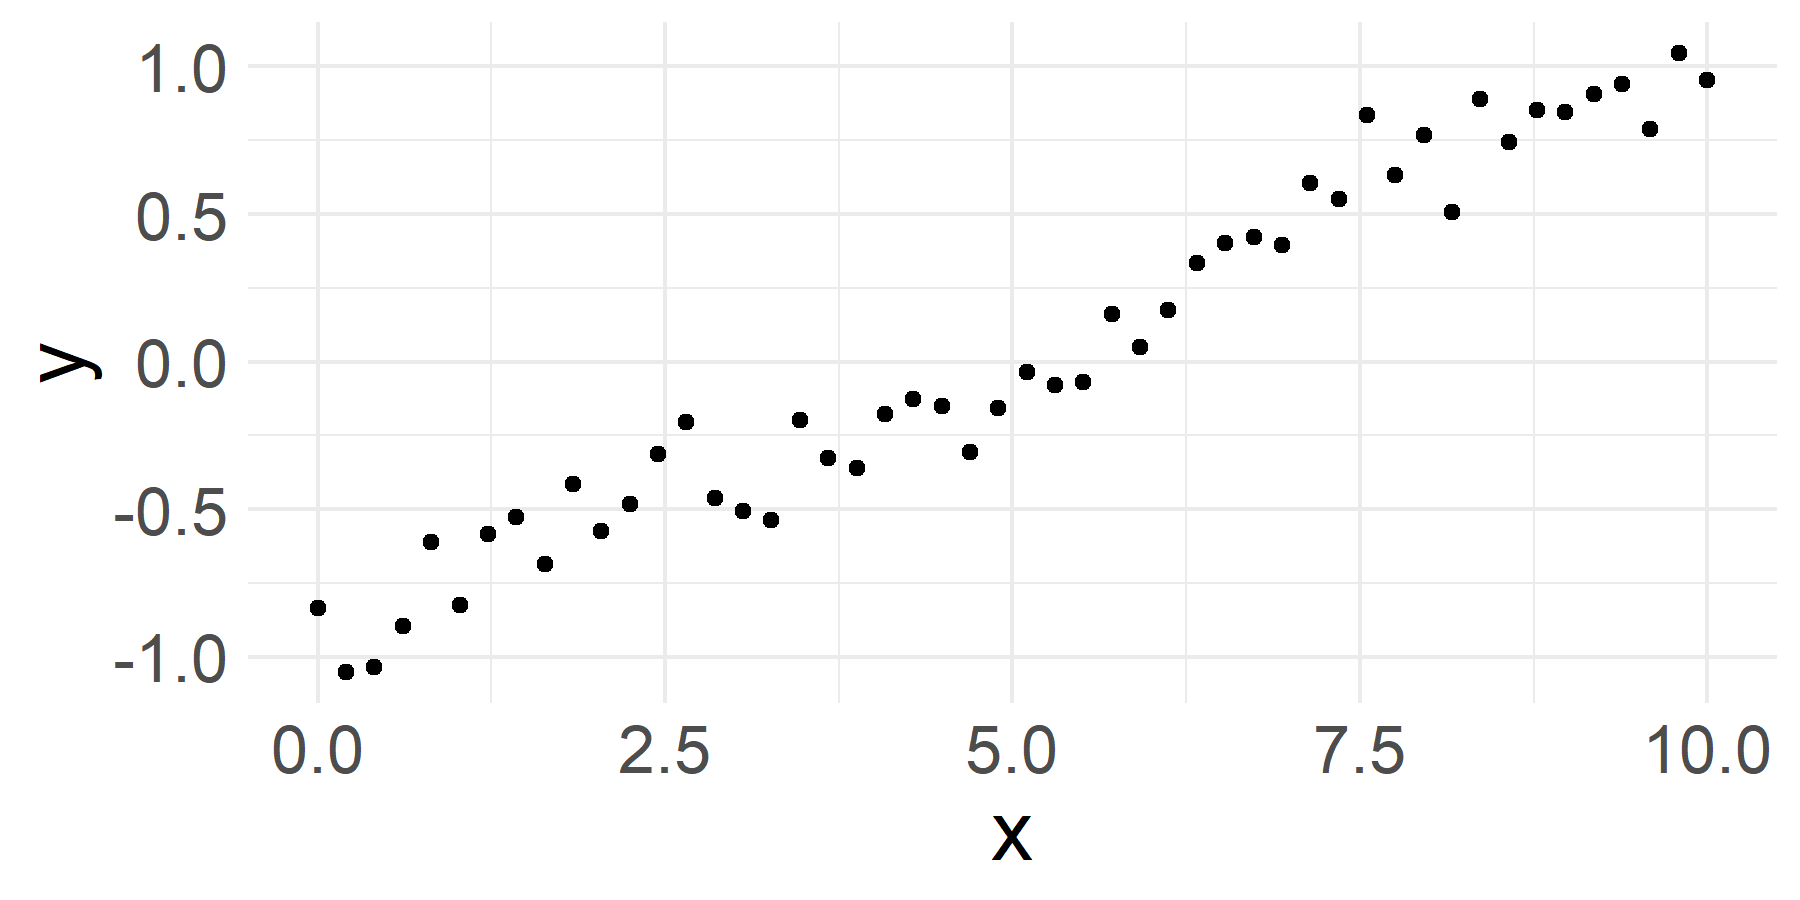
\includegraphics[width = 0.45\textwidth]{figure/illustration_data_normal.png}
\end{figure}

\framebreak

% ------------------------------------------------------------------------------

\begin{enumerate}
  \item We start with the simplest model, the optimal constant -- mean of the 
  target variable in the case of $L2$ loss and median in the case of $L1$ loss.
  \item We improve the model by calculating the pointwise 
  pseudo-residuals on the training data, and fit a GAM on the residuals.
  \begin{enumerate}
    \item The GAM base learners model the conditional mean via cubic $B$-splines 
    with 40 knots. 
    % i.e., $\bmmxth = \sum_{k = 1}^{K + \ell} B_k^{(3)}(\xv)$, with $\ell = 3$ 
    % and $K = 40$ knots.
    \item In each step, the GAM fitted on the current pseudo-residuals is
    multiplied by a constant learning rate of $0.2$ and added to the previous
    model.
    \item This procedure is repeated multiple times.
  \end{enumerate}
\end{enumerate}

\end{vbframe}

% ------------------------------------------------------------------------------

\begin{frame}{GAM with $L2$ VS $L1$ loss}

Top: $L2$ loss, bottom: $L1$ loss

\vfill

% \begin{center}
\only<1>{ 
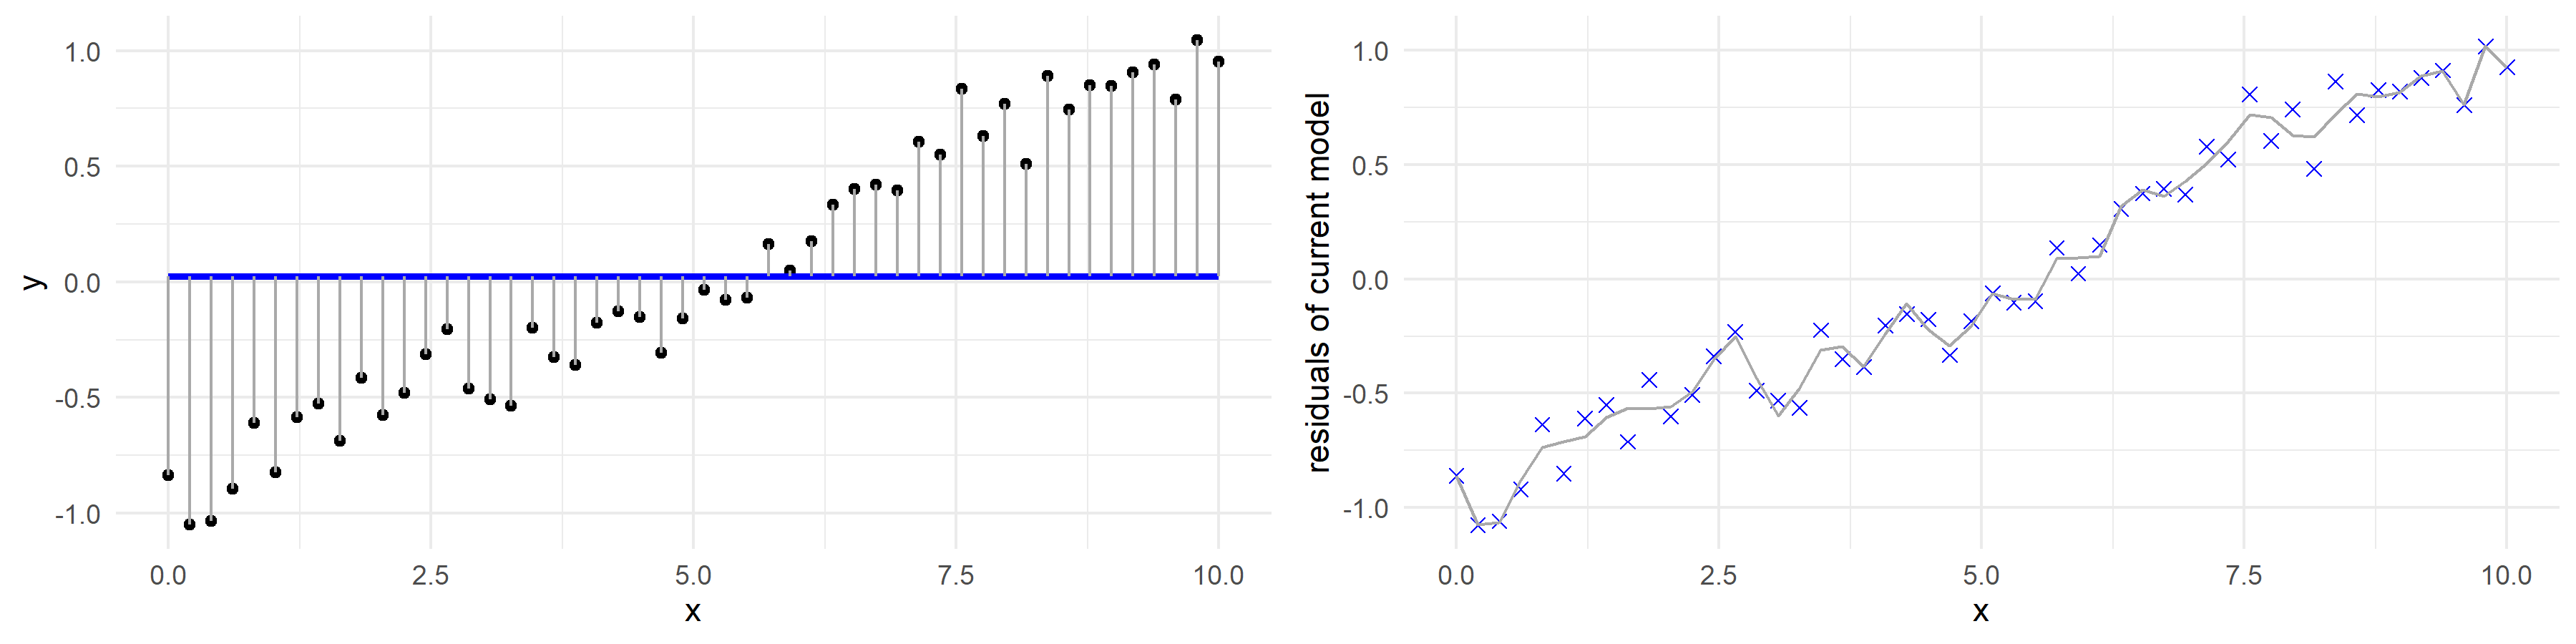
\includegraphics[width=\textwidth]{figure/illustration_gaussian_L2_1.png}
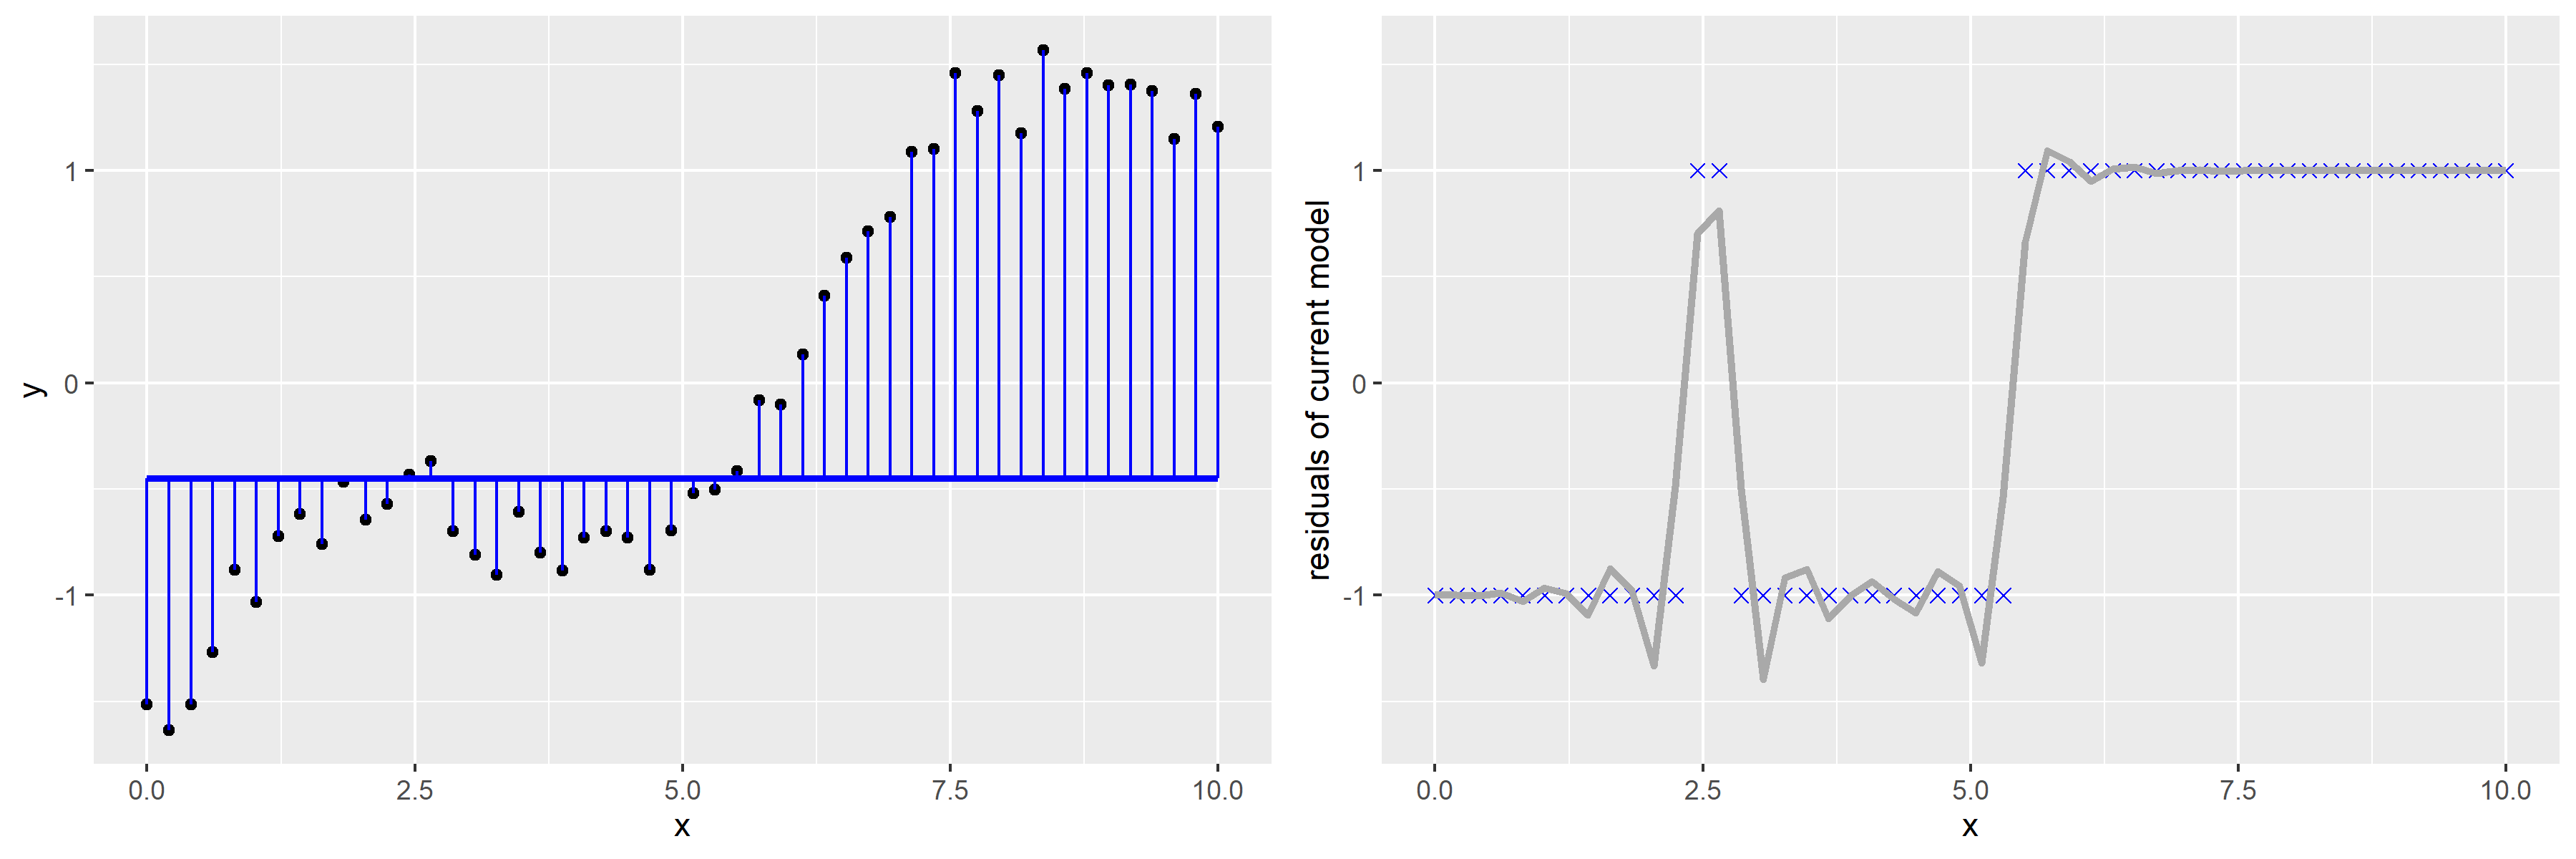
\includegraphics[width=\textwidth]{figure/illustration_gaussian_L1_1.png}

\vfill

Iteration 1

}

\only<2>{ 
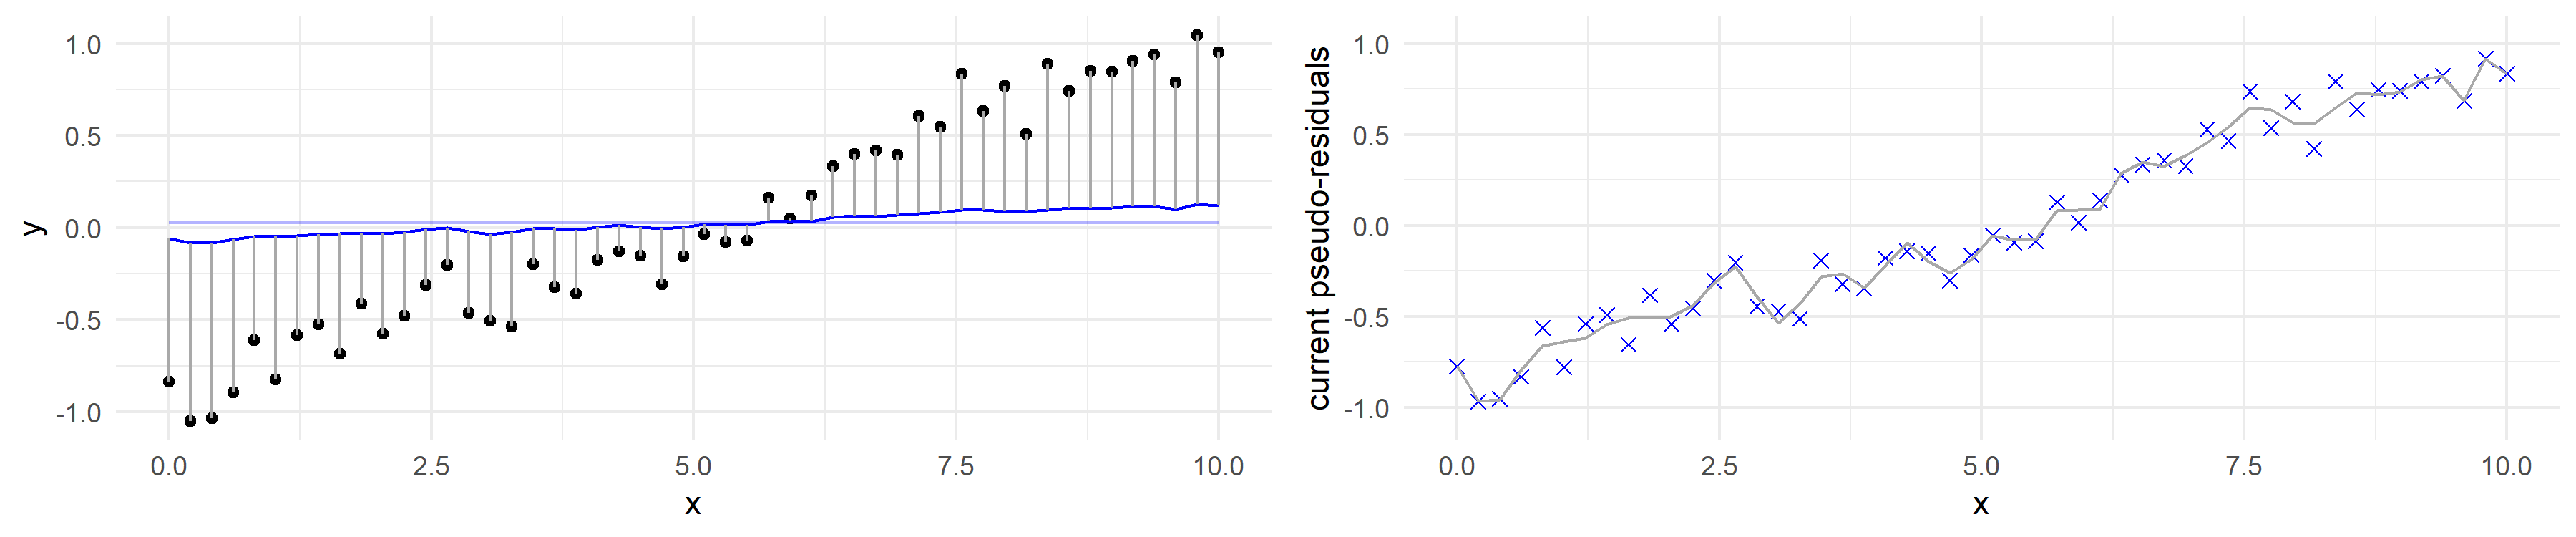
\includegraphics[width=\textwidth]{figure/illustration_gaussian_L2_2.png}
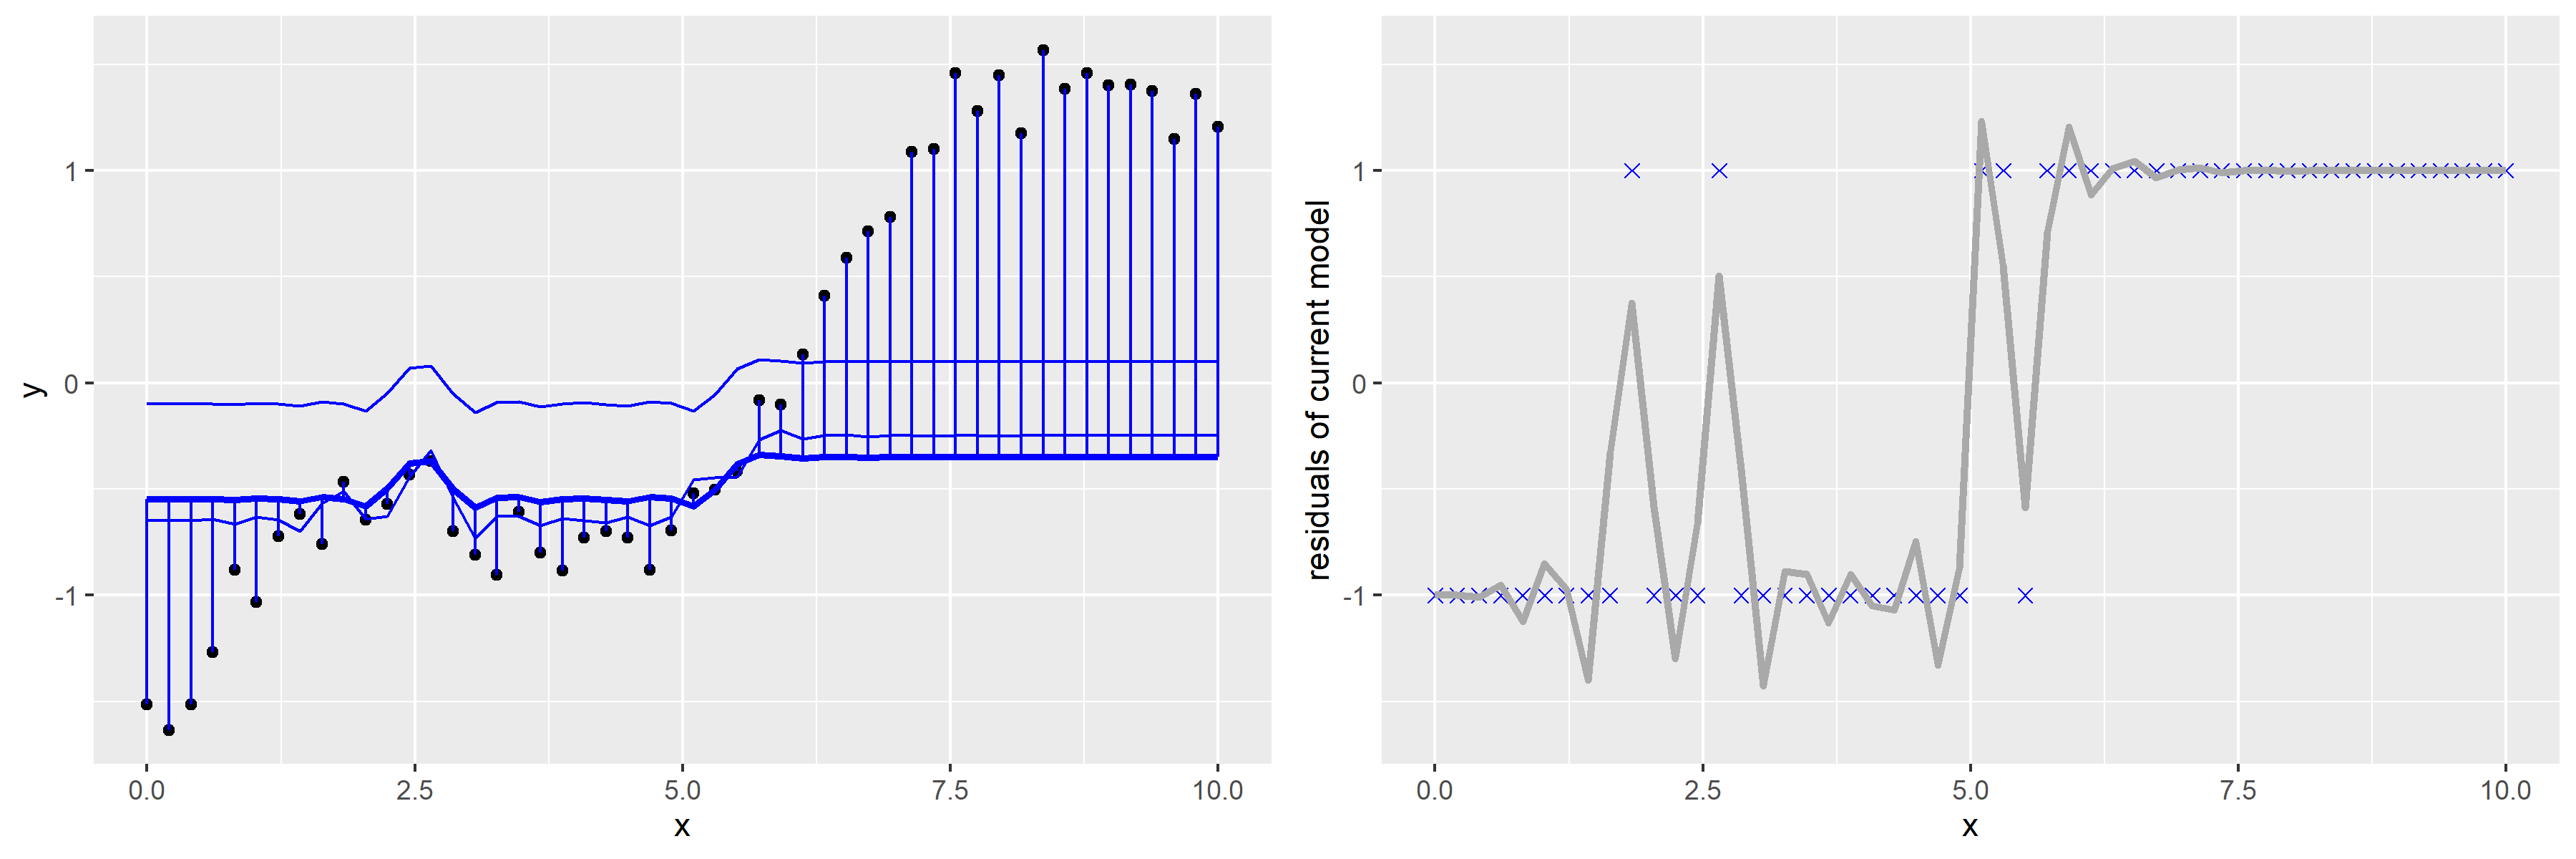
\includegraphics[width=\textwidth]{figure/illustration_gaussian_L1_2.png}

\vfill

Iteration 2
}
\only<3>{ 
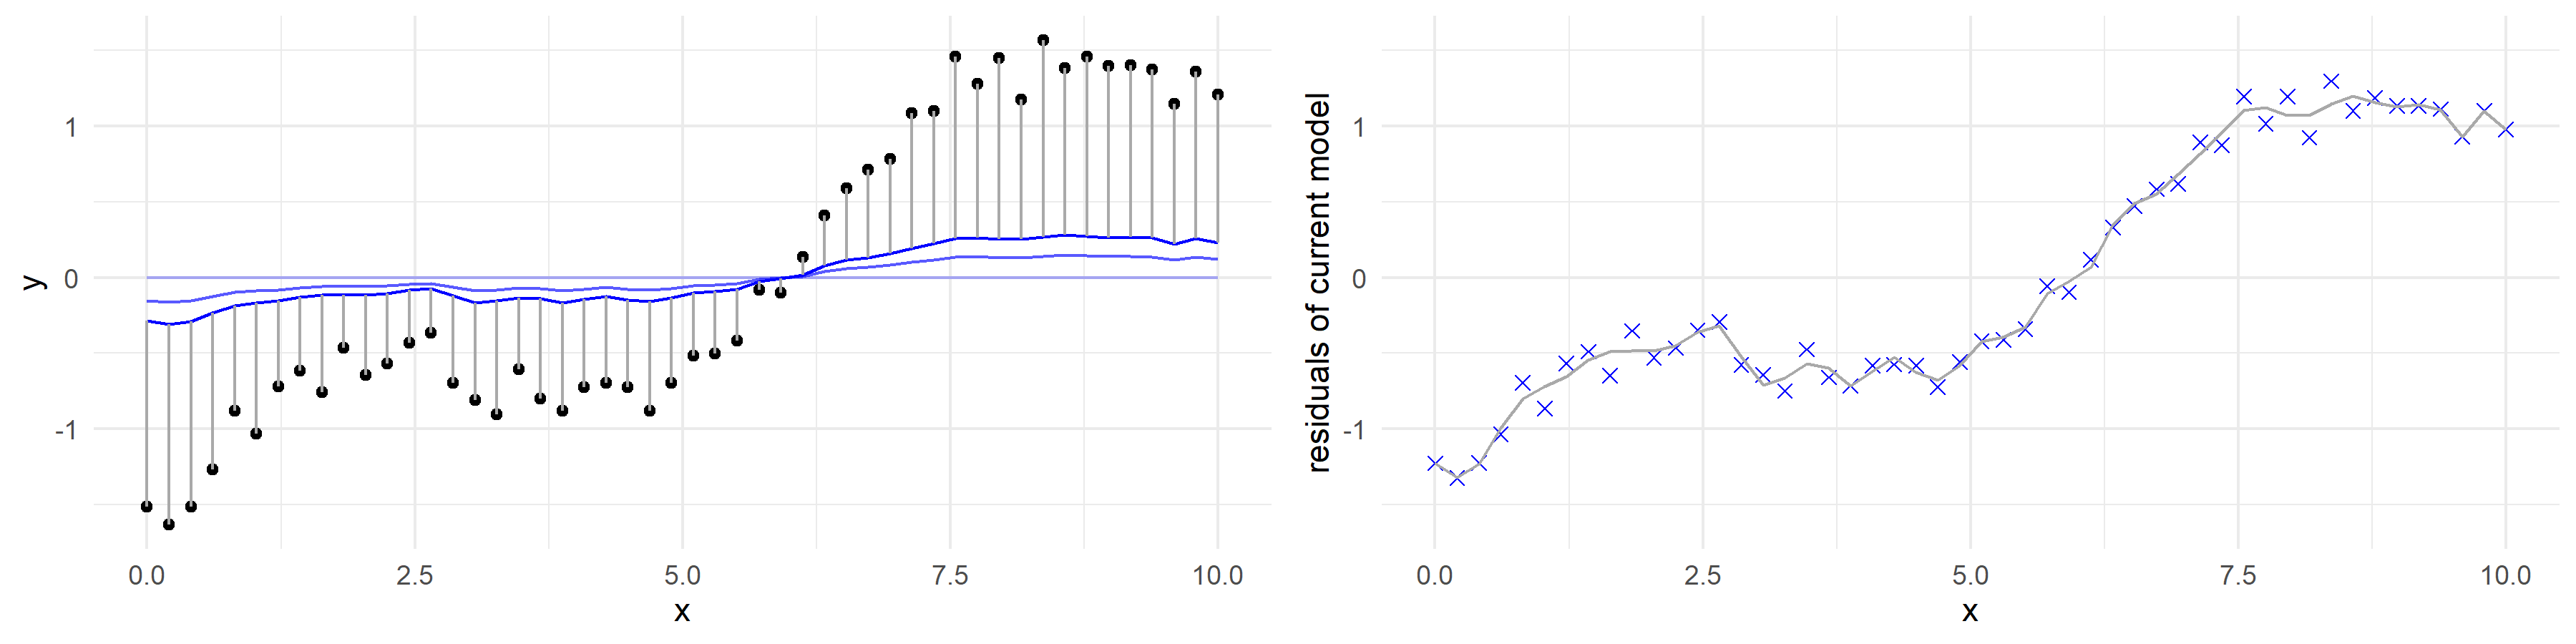
\includegraphics[width=\textwidth]{figure/illustration_gaussian_L2_3.png}
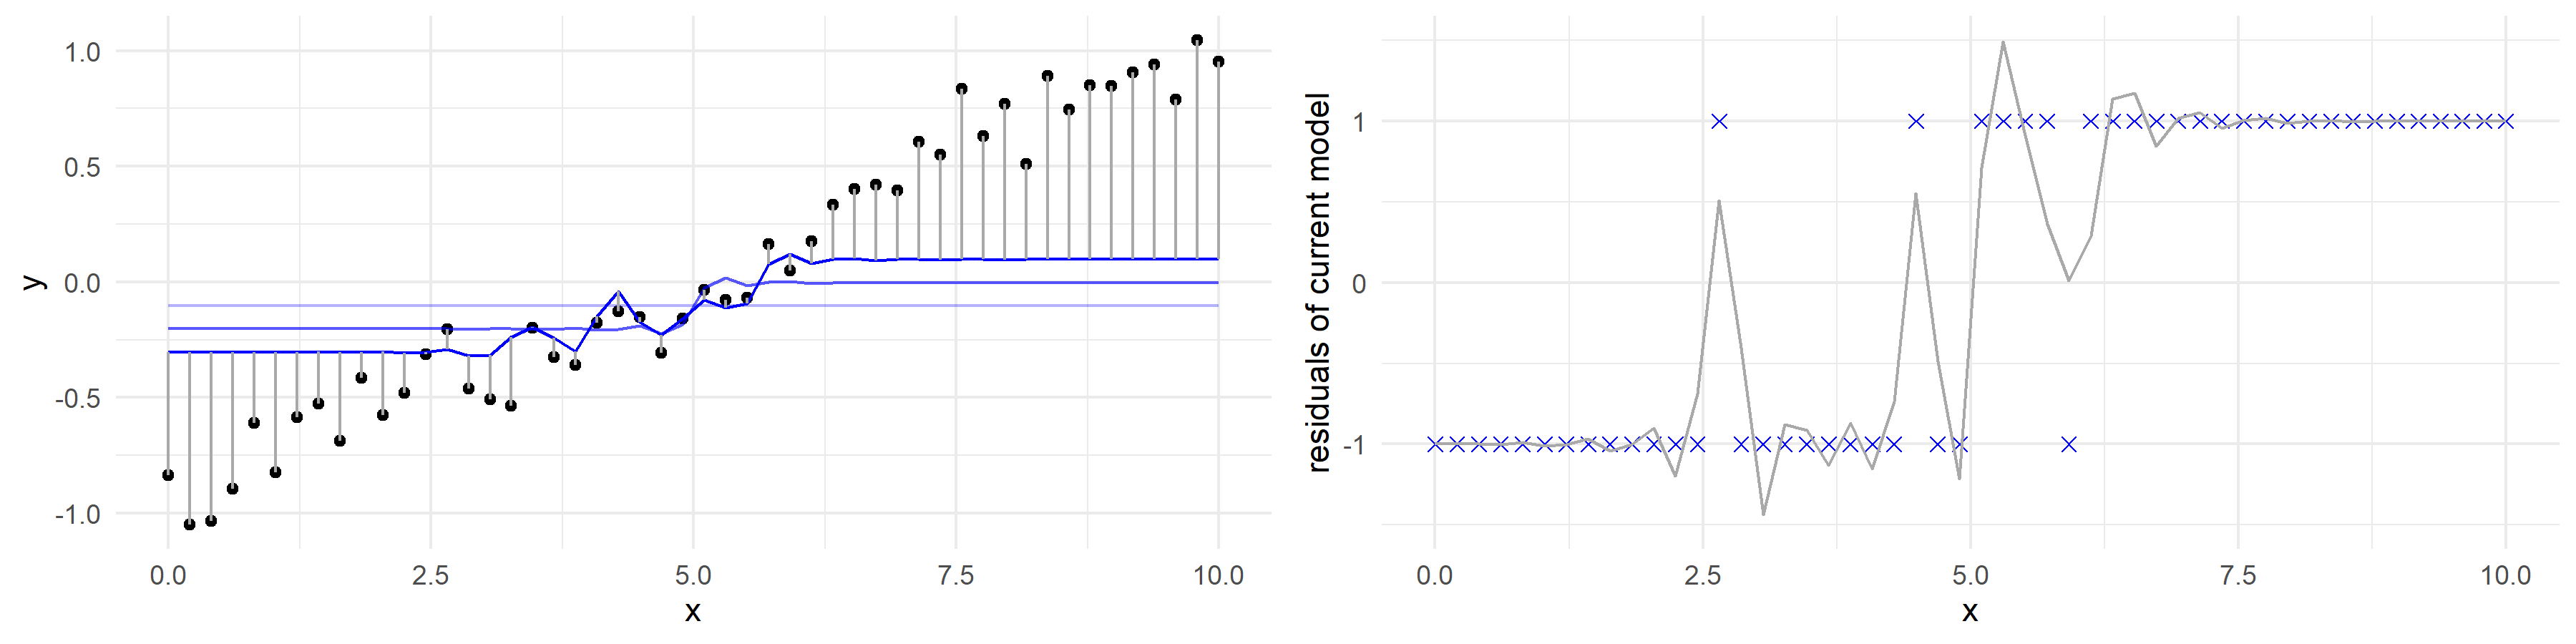
\includegraphics[width=\textwidth]{figure/illustration_gaussian_L1_3.png}

\vfill

Iteration 3
}
\only<4>{ 
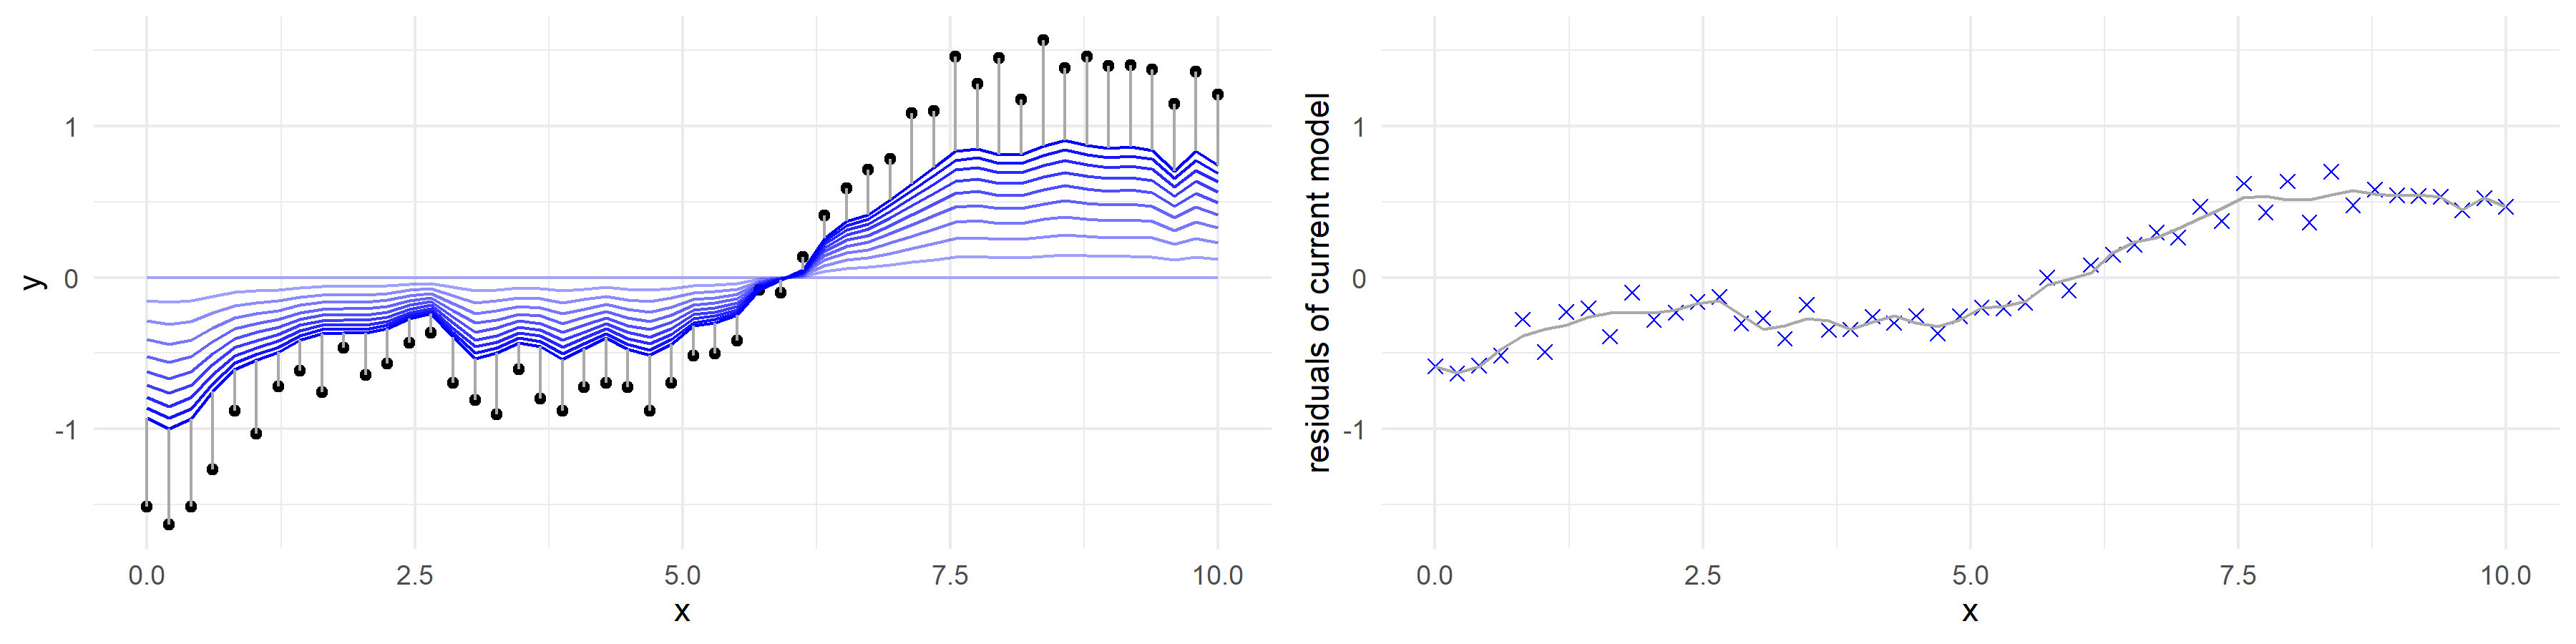
\includegraphics[width=\textwidth]{figure/illustration_gaussian_L2_10.png}
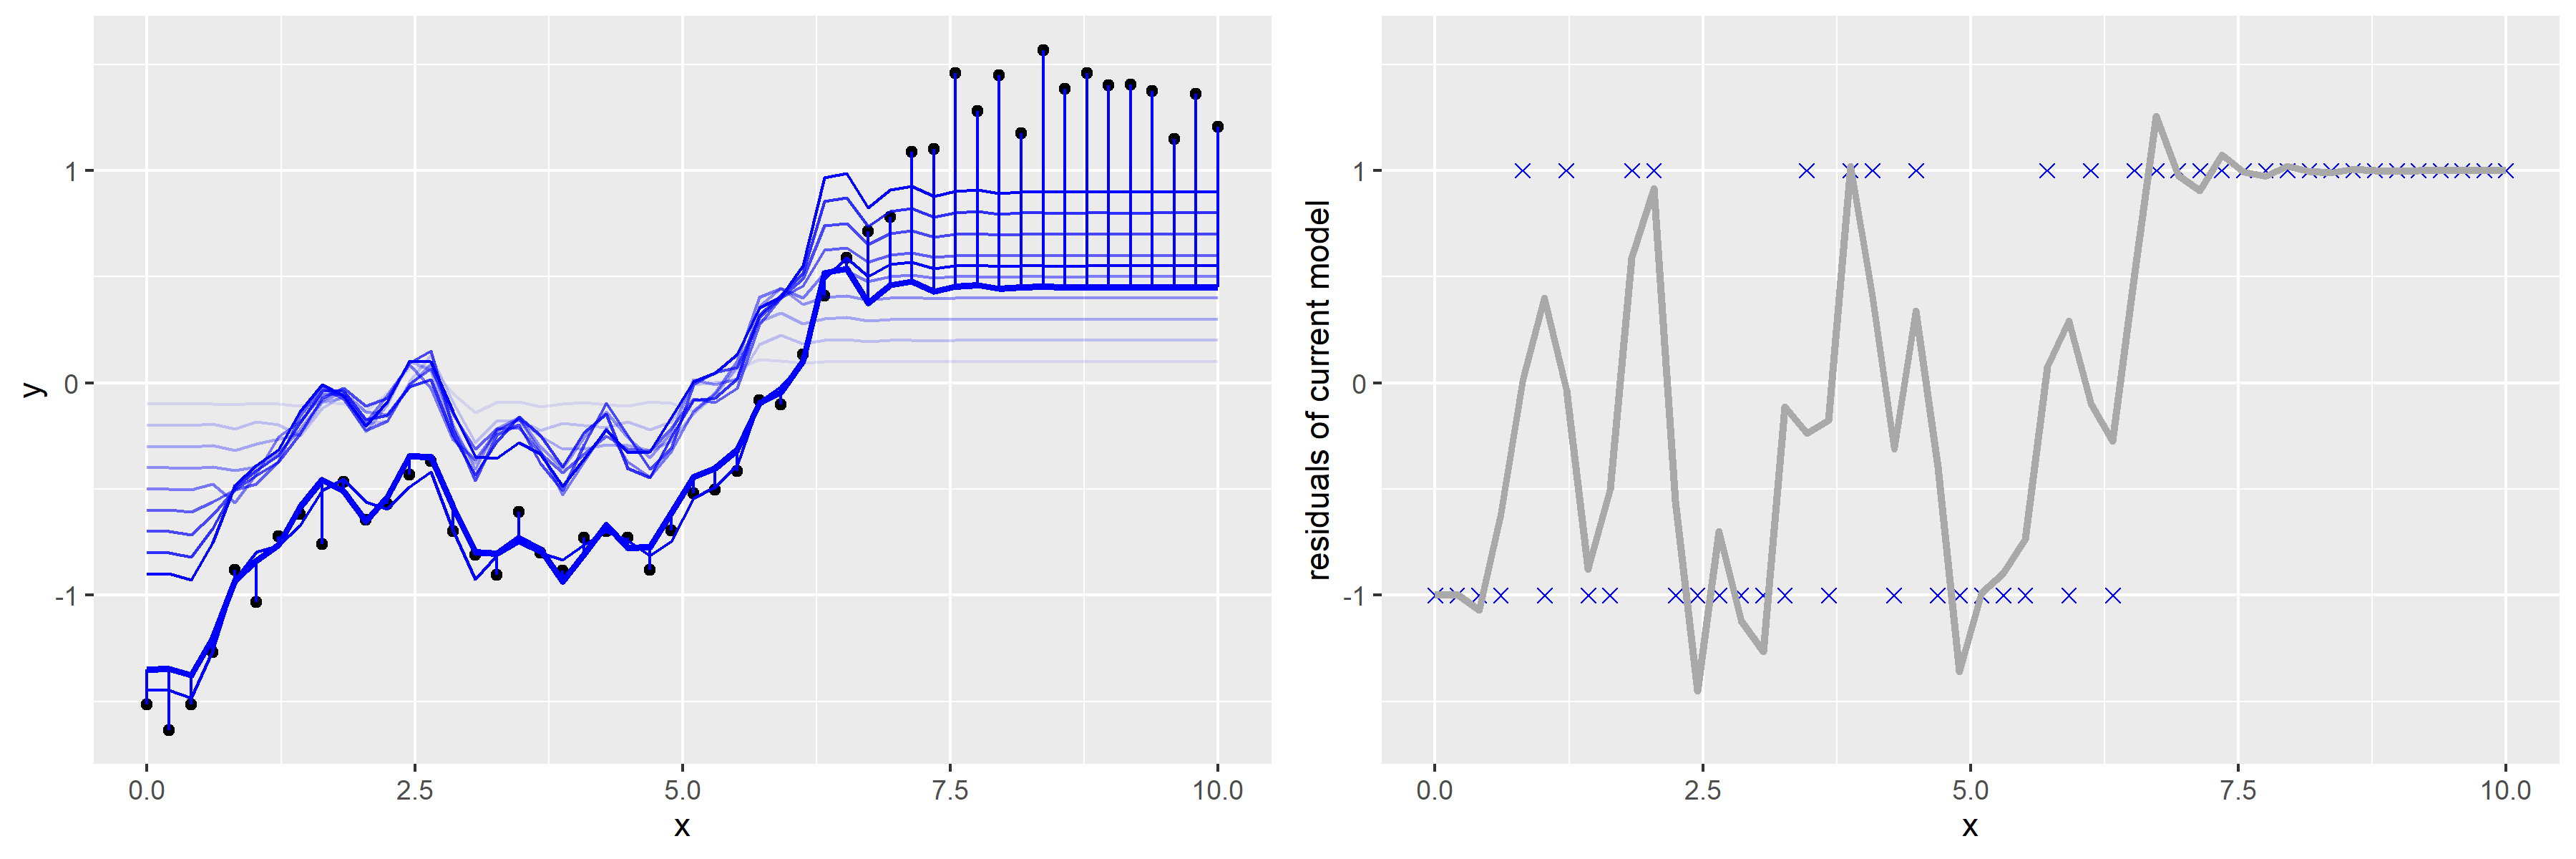
\includegraphics[width=\textwidth]{figure/illustration_gaussian_L1_10.png}

\vfill

Iteration 10
}

\only<5>{ 
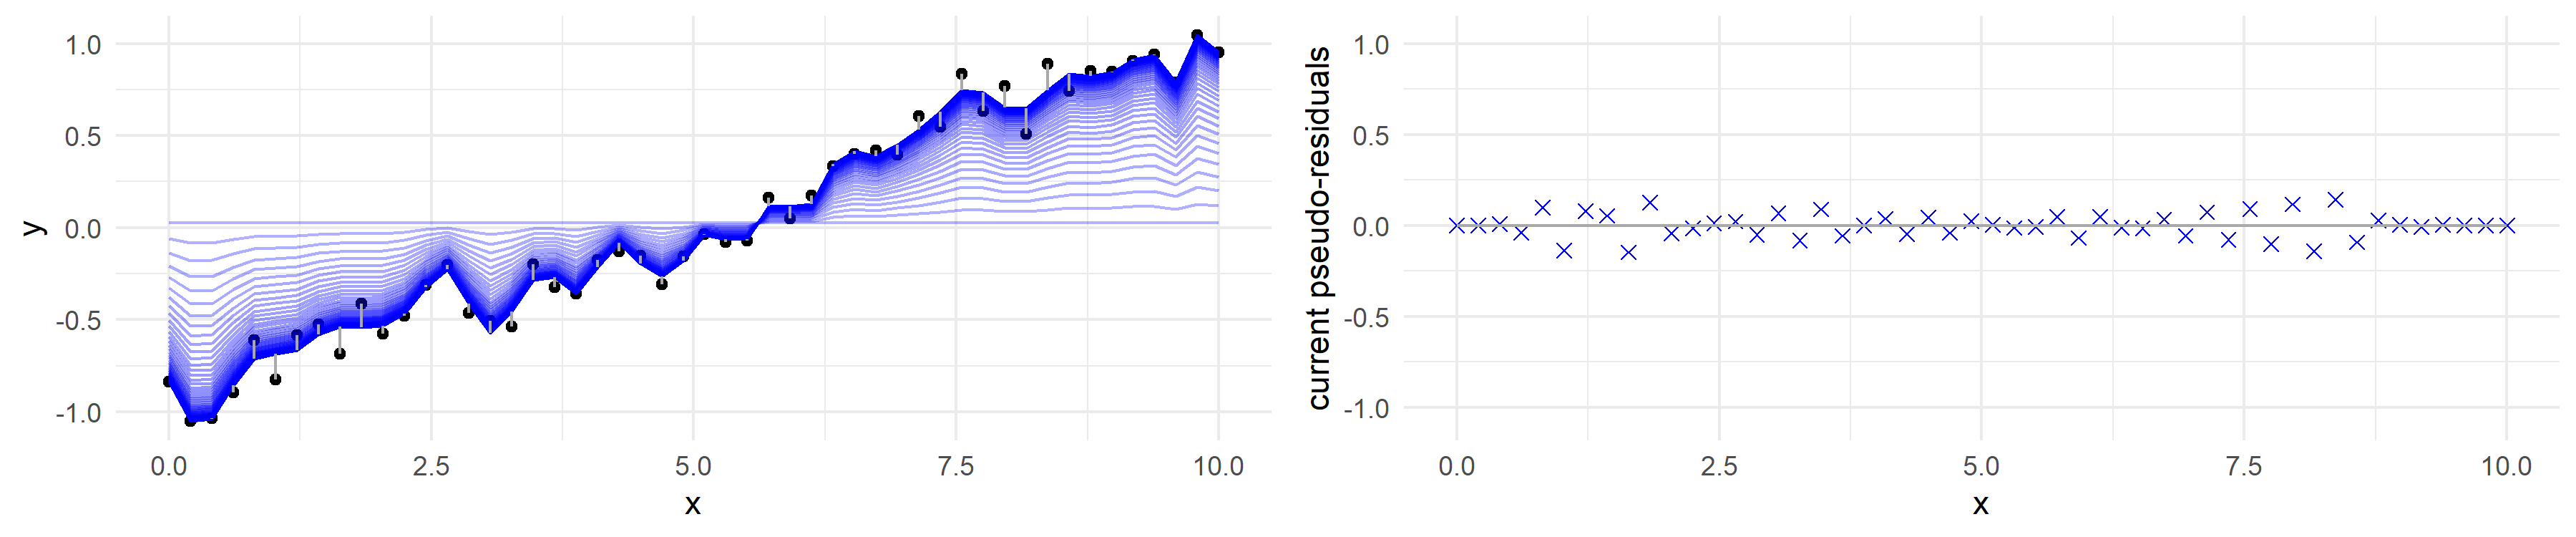
\includegraphics[width=\textwidth]{figure/illustration_gaussian_L2_100.png}
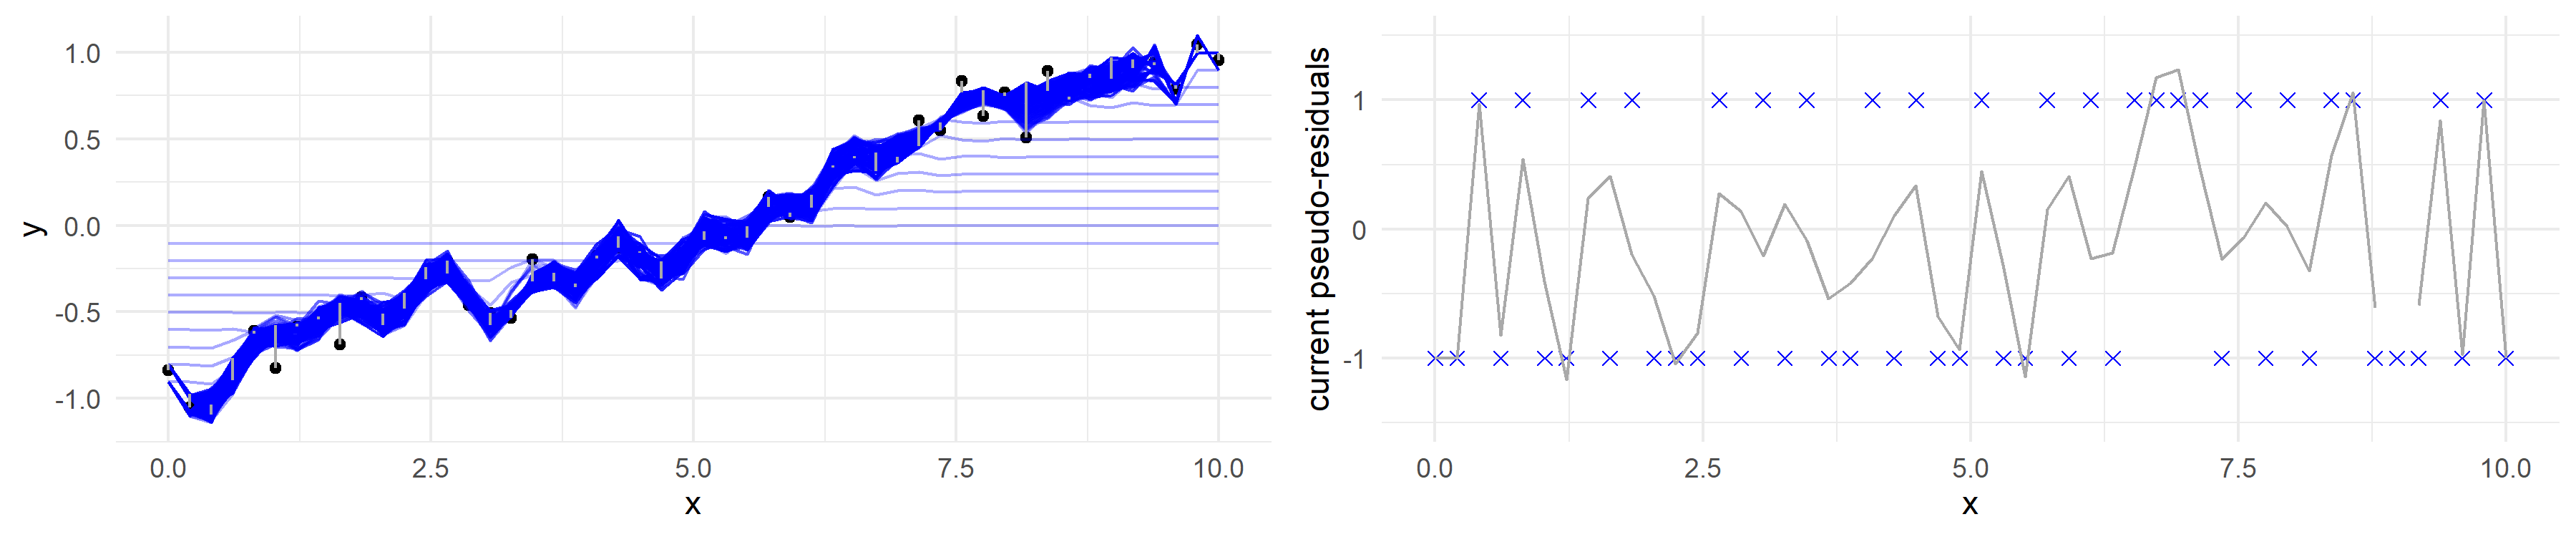
\includegraphics[width=\textwidth]{figure/illustration_gaussian_L1_100.png}

\vfill

Iteration 100
}

\vfill

\footnotesize

The nature of the pseudo-residuals affects gradual model fit: as $L1$ only 
considers residuals' sign, the corresponding base learners are less affected by very large or small values
compared to $L2$ and hence lead to more moderate changes.%'s approximation of ever smaller residuals.

\end{frame}

% ------------------------------------------------------------------------------

\begin{frame}{GAM with Huber loss}
We can also use Huber loss, which is closer to $L2$ for large $\delta$ values 
and closer to $L1$ for 
smaller $\delta$ values. Top: $\delta$ = 2, bottom: $\delta$ = 0.2.

\vfill

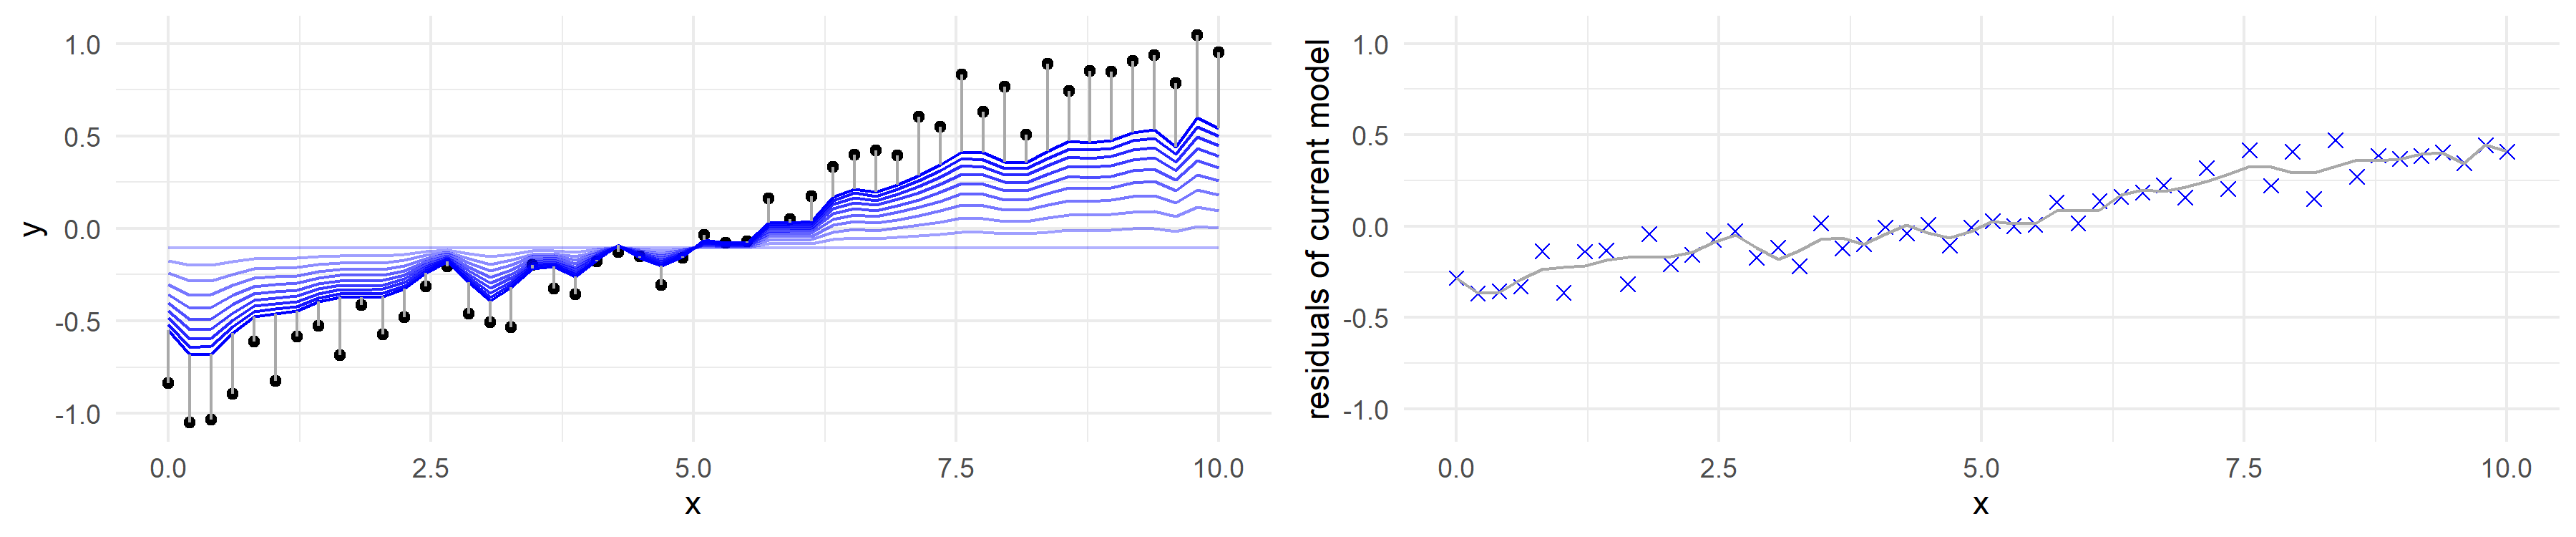
\includegraphics[width=\textwidth]{figure/illustration_gaussian_huber_2_10.png}
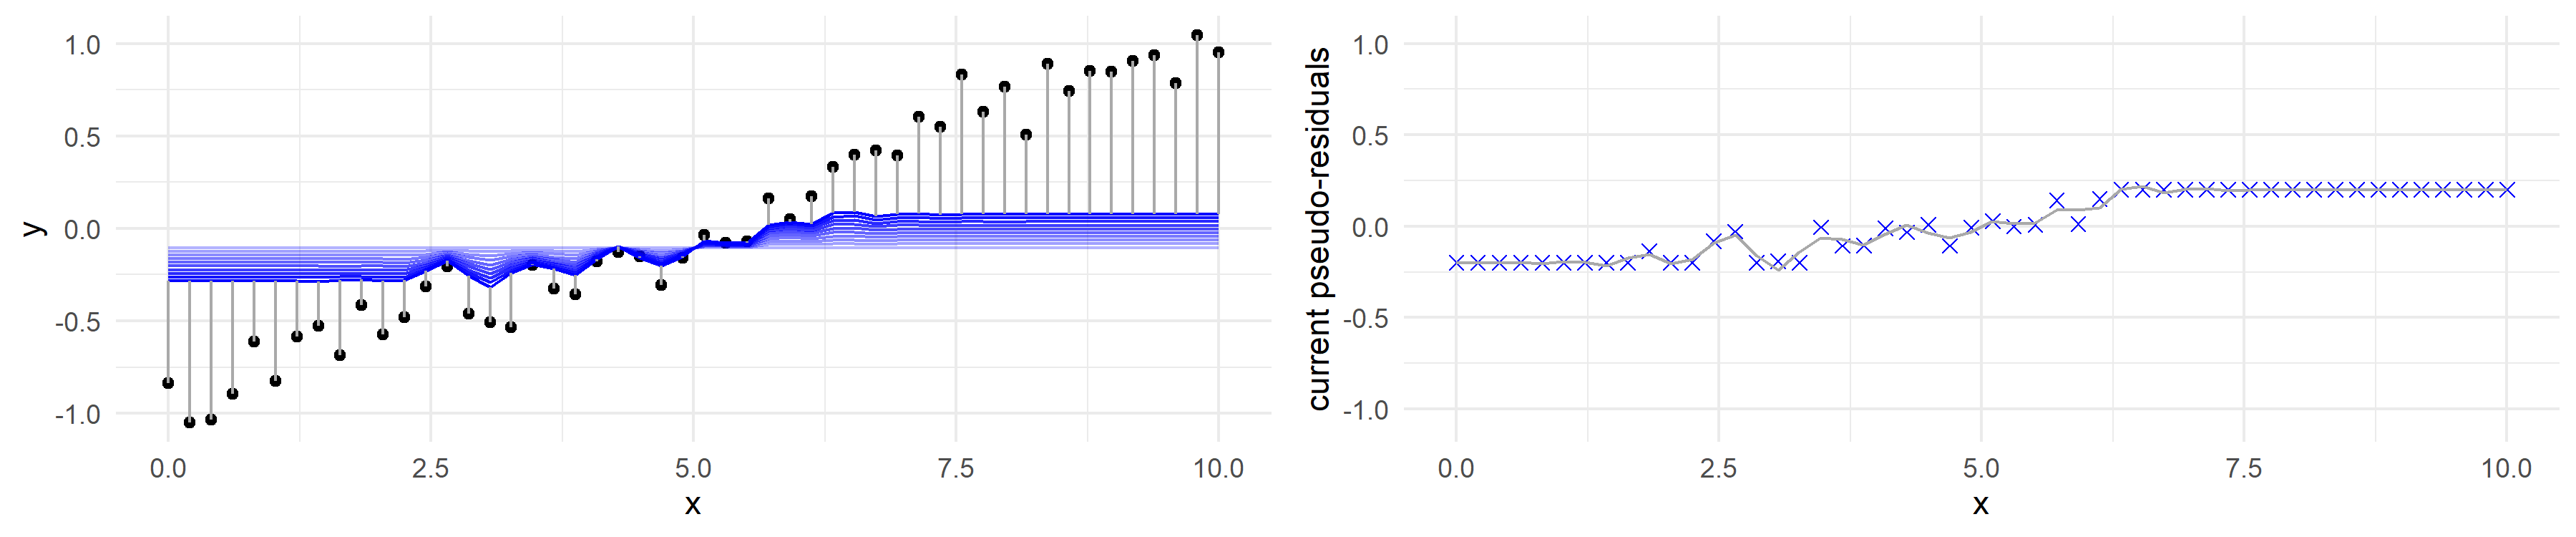
\includegraphics[width=\textwidth]{figure/illustration_gaussian_huber_02_10.png}

\vfill

Iteration 10

%\vfill

\footnotesize
\begin{columns}[c]
\begin{column}{0.75\textwidth}
We see how for smaller $\delta$ (bottom) pseudo-residuals are often effectively
bounded, resulting in $L1$-like behavior, while the upper plot more closely 
resembles $L2$ loss.
\end{column}
\begin{column}{0.24\textwidth}
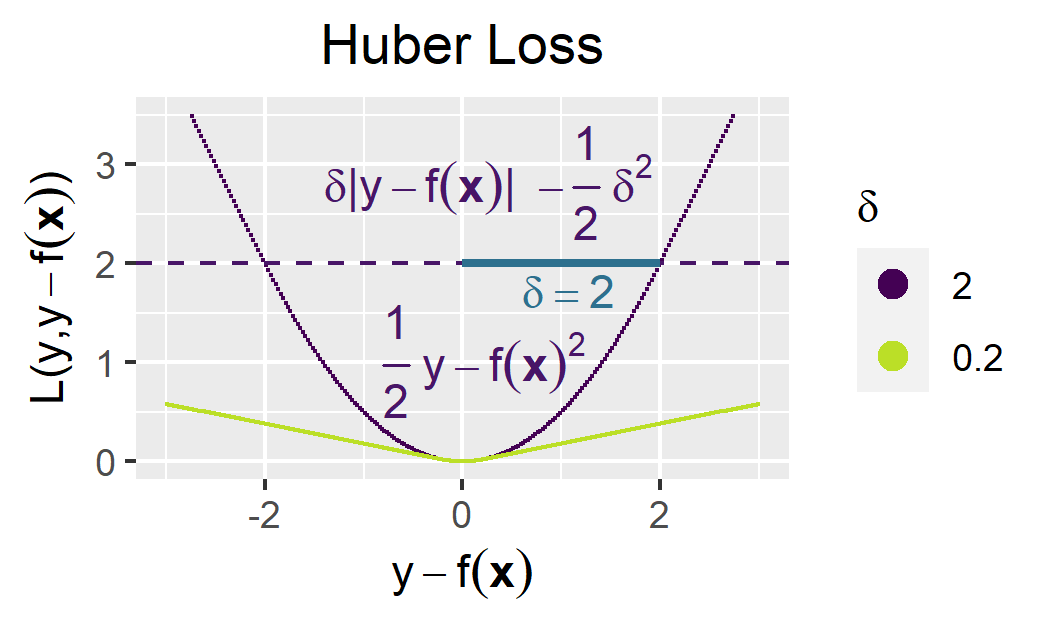
\includegraphics[width=1.2\textwidth]{figure/fig-loss-huber-delta.png}
\end{column}
\end{columns}
% The lower right plot shows that pseudo-residuals often take values of the upper and lower
% bounds (depending on $\delta$) and thus the behaviour is closer to the $L1$ loss while the upper plots show a
% similar behavior to the $L2$ loss. 

\end{frame}

% ------------------------------------------------------------------------------

\begin{frame}{GAM with outliers}
Instead of normally distributed noise we can assume a $t$-distribution, leading 
to outliers in the observed target values.
Top: $L2$, bottom: $L1$.

\vfill

\only<1>{ 
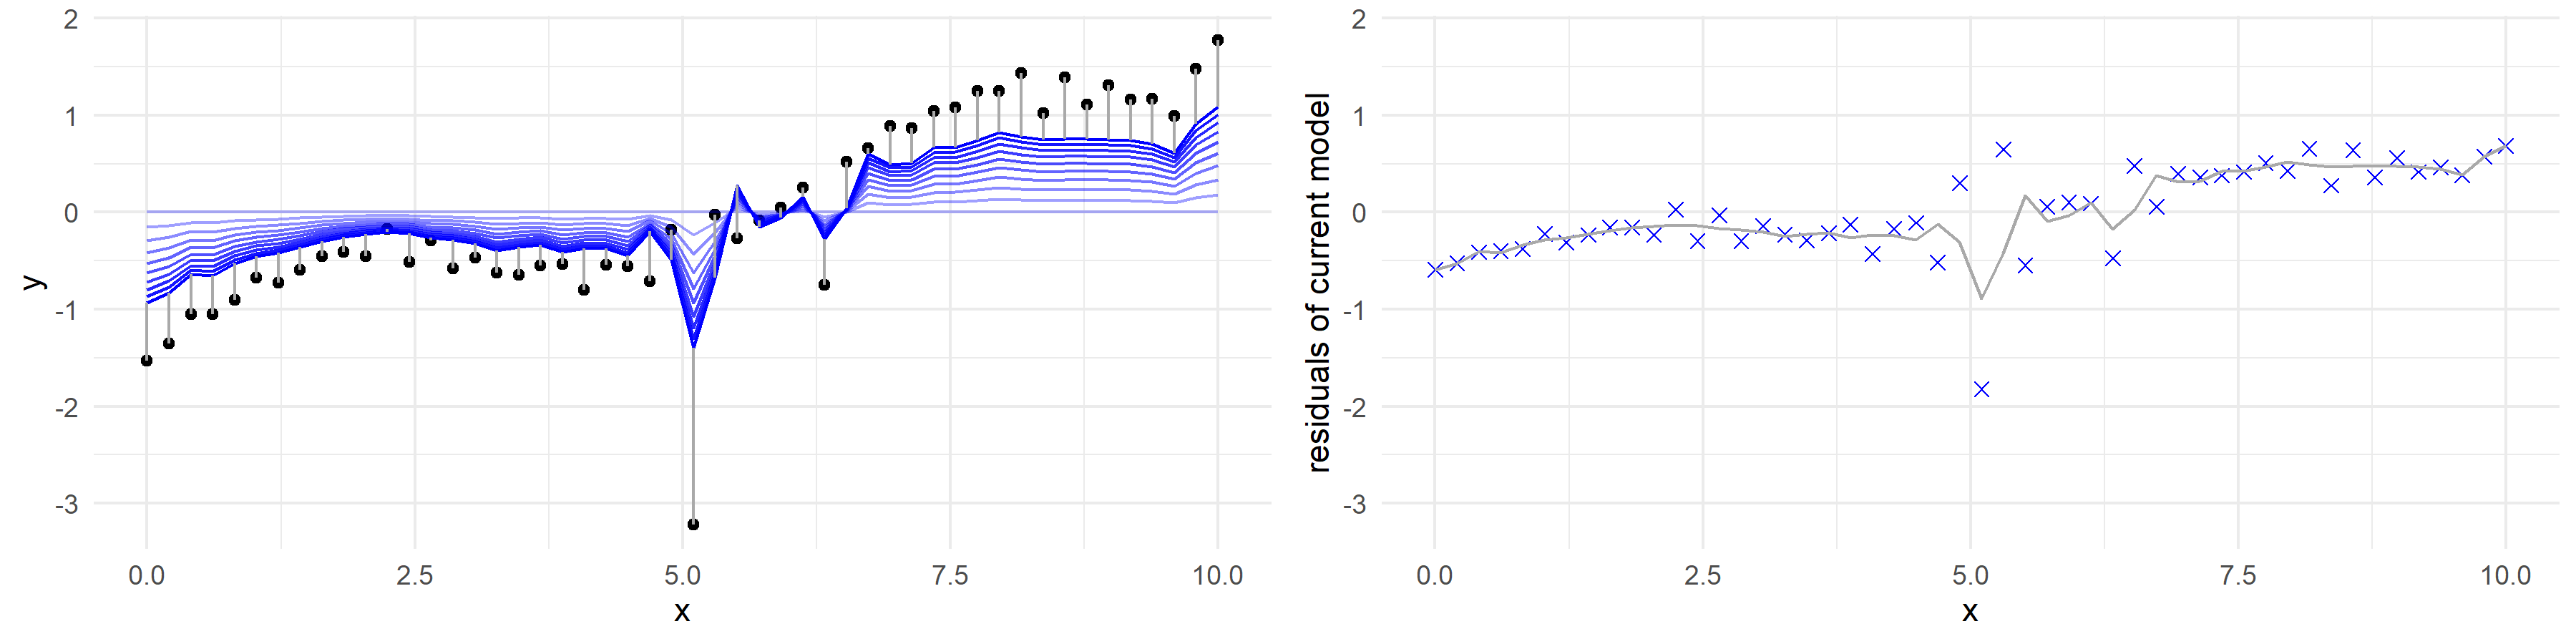
\includegraphics[width=\textwidth]{figure/illustration_tdist_L2_10.png}
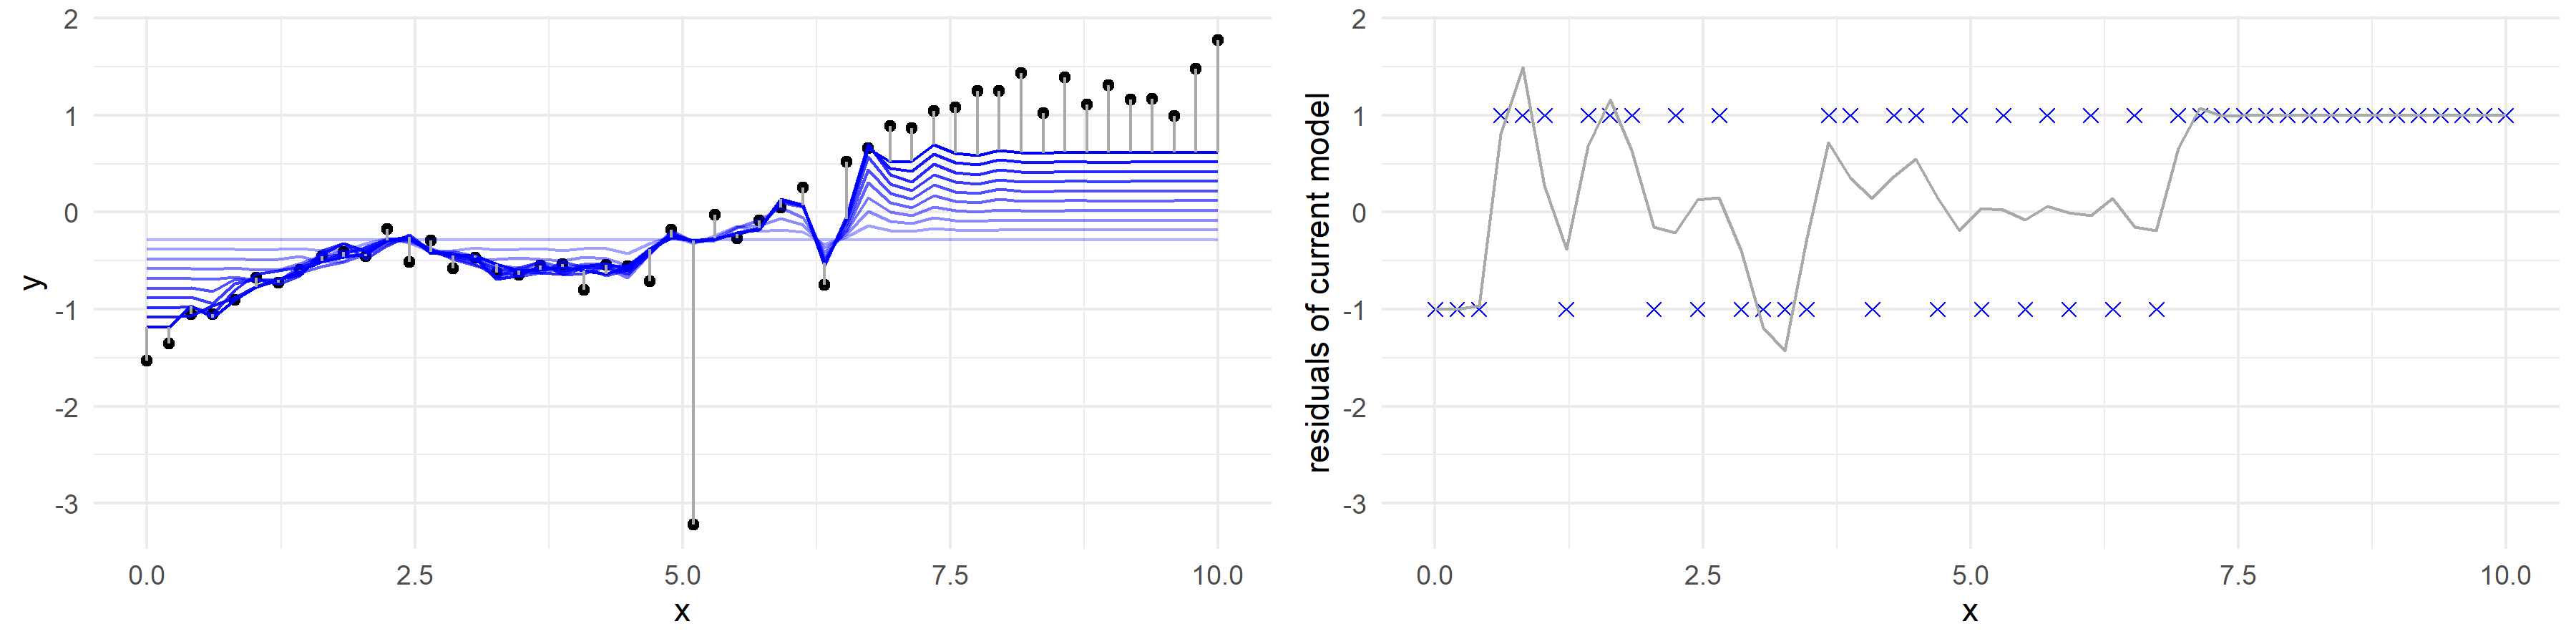
\includegraphics[width=\textwidth]{figure/illustration_tdist_L1_10.png}

\vfill
Iteration 10
}
\only<2>{ 
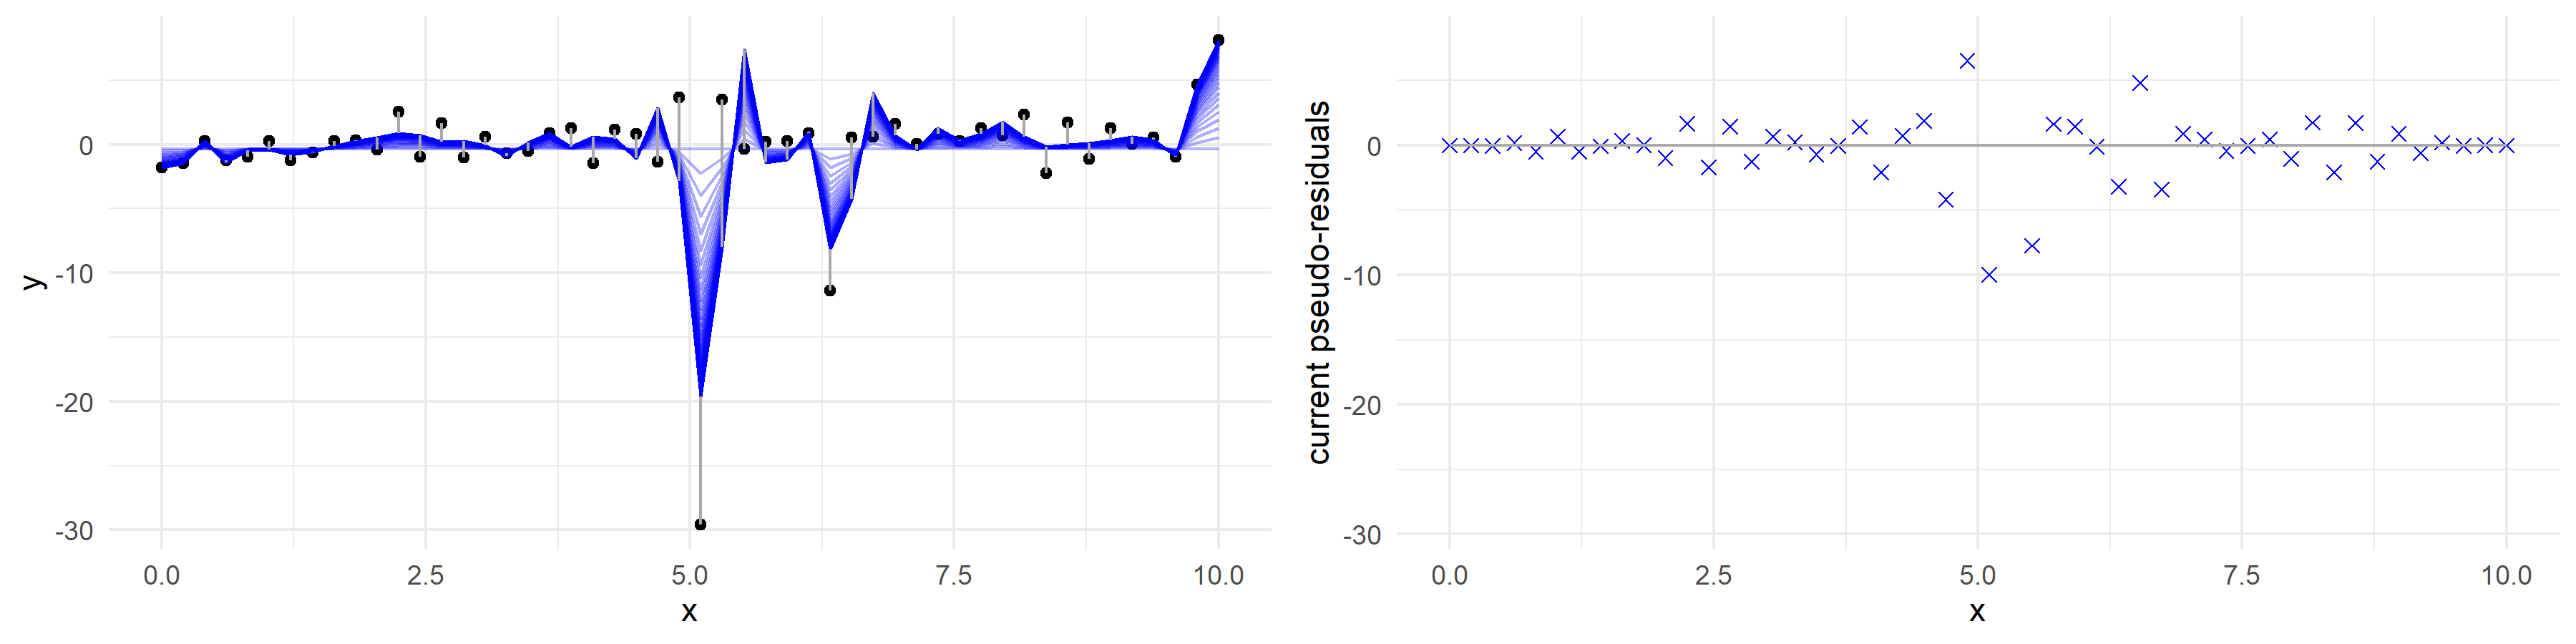
\includegraphics[width=\textwidth]{figure/illustration_tdist_L2_100.png}
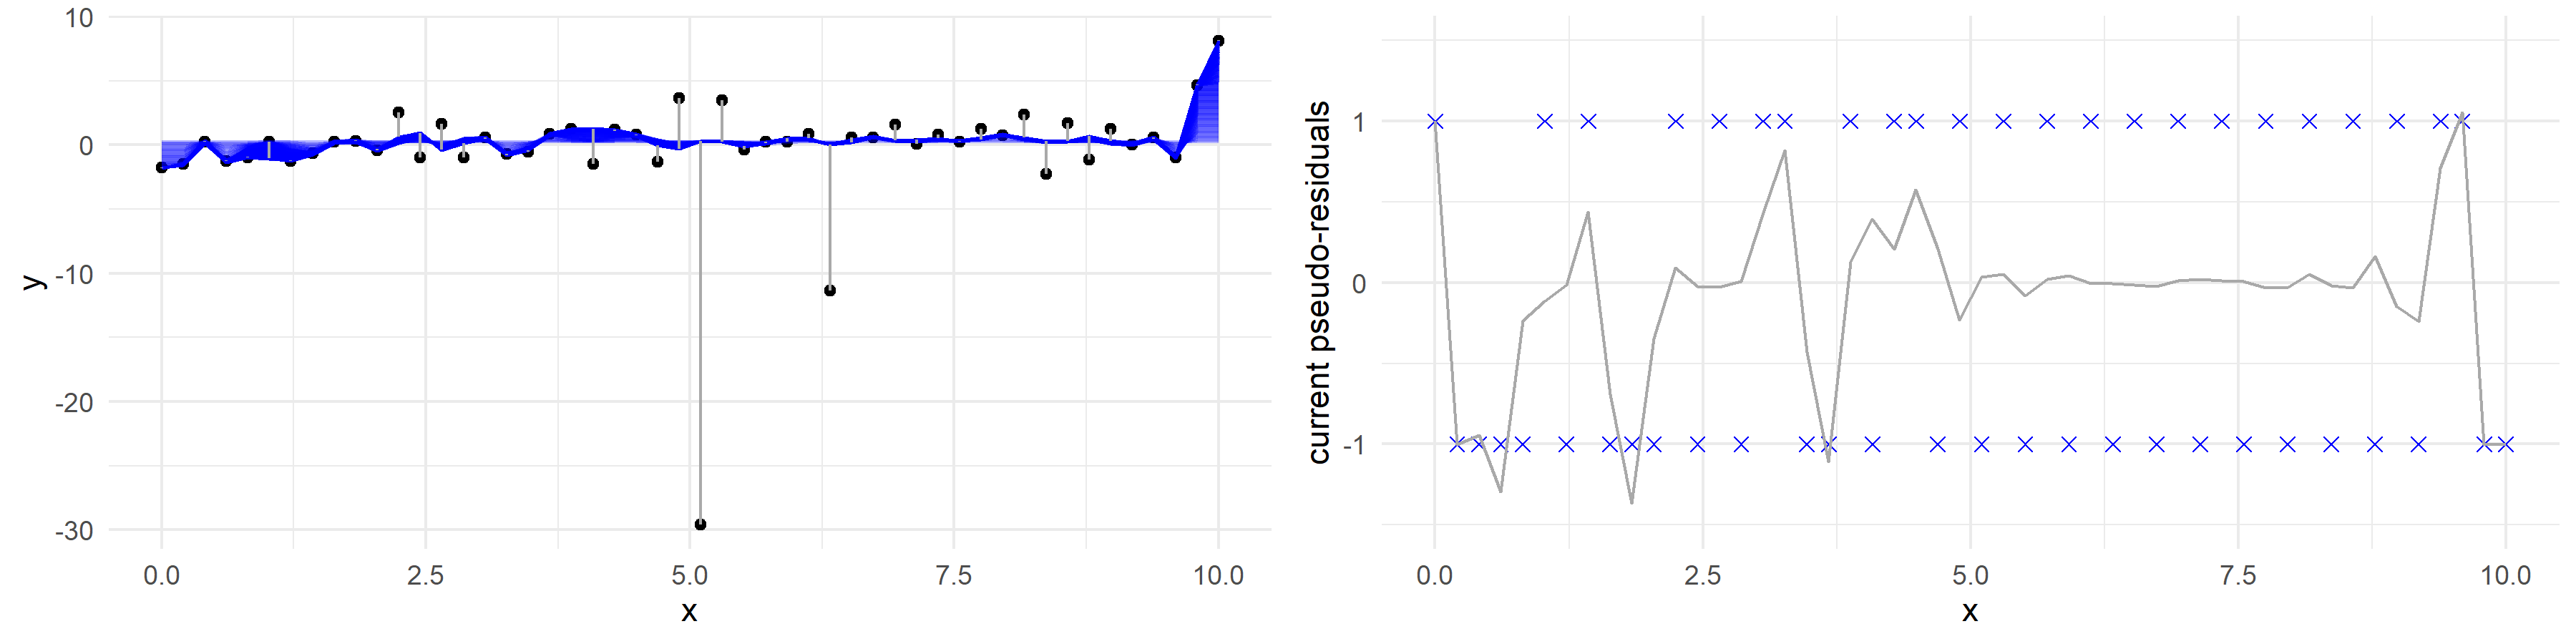
\includegraphics[width=\textwidth]{figure/illustration_tdist_L1_100.png}

\vfill
Iteration 100
}

\vfill

\footnotesize

$L2$ loss is affected by outliers rather strongly, whereas $L1$ solely considers 
residuals' sign and not their magnitude, resulting in a more robust model.

\end{frame}

% ------------------------------------------------------------------------------

\begin{frame}{LM with $L2$ vs $L1$ loss}
Instead of using a GAM as base learner we now use a simple linear model.
% It follows that this is equivalent to applying gradient descent on linear 
% regression.
Top: $L2$, bottom: $L1$.

\vfill

\only<1>{ 
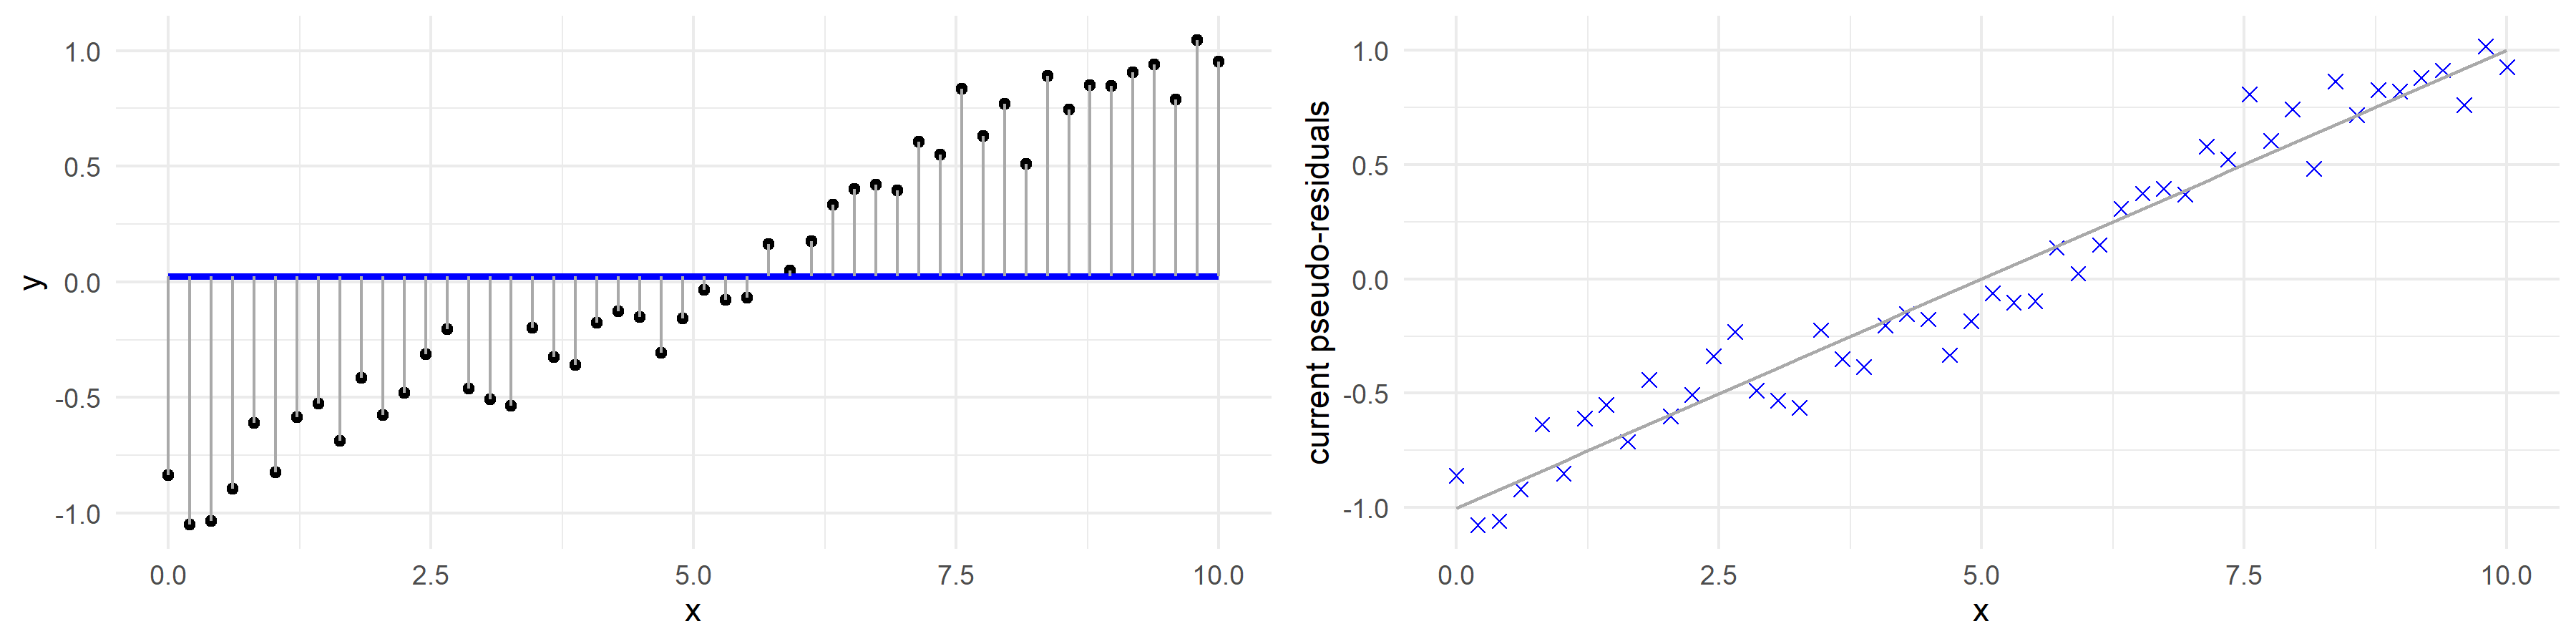
\includegraphics[width=\textwidth]{figure/illustration_gaussian_L2_lin_1.png}
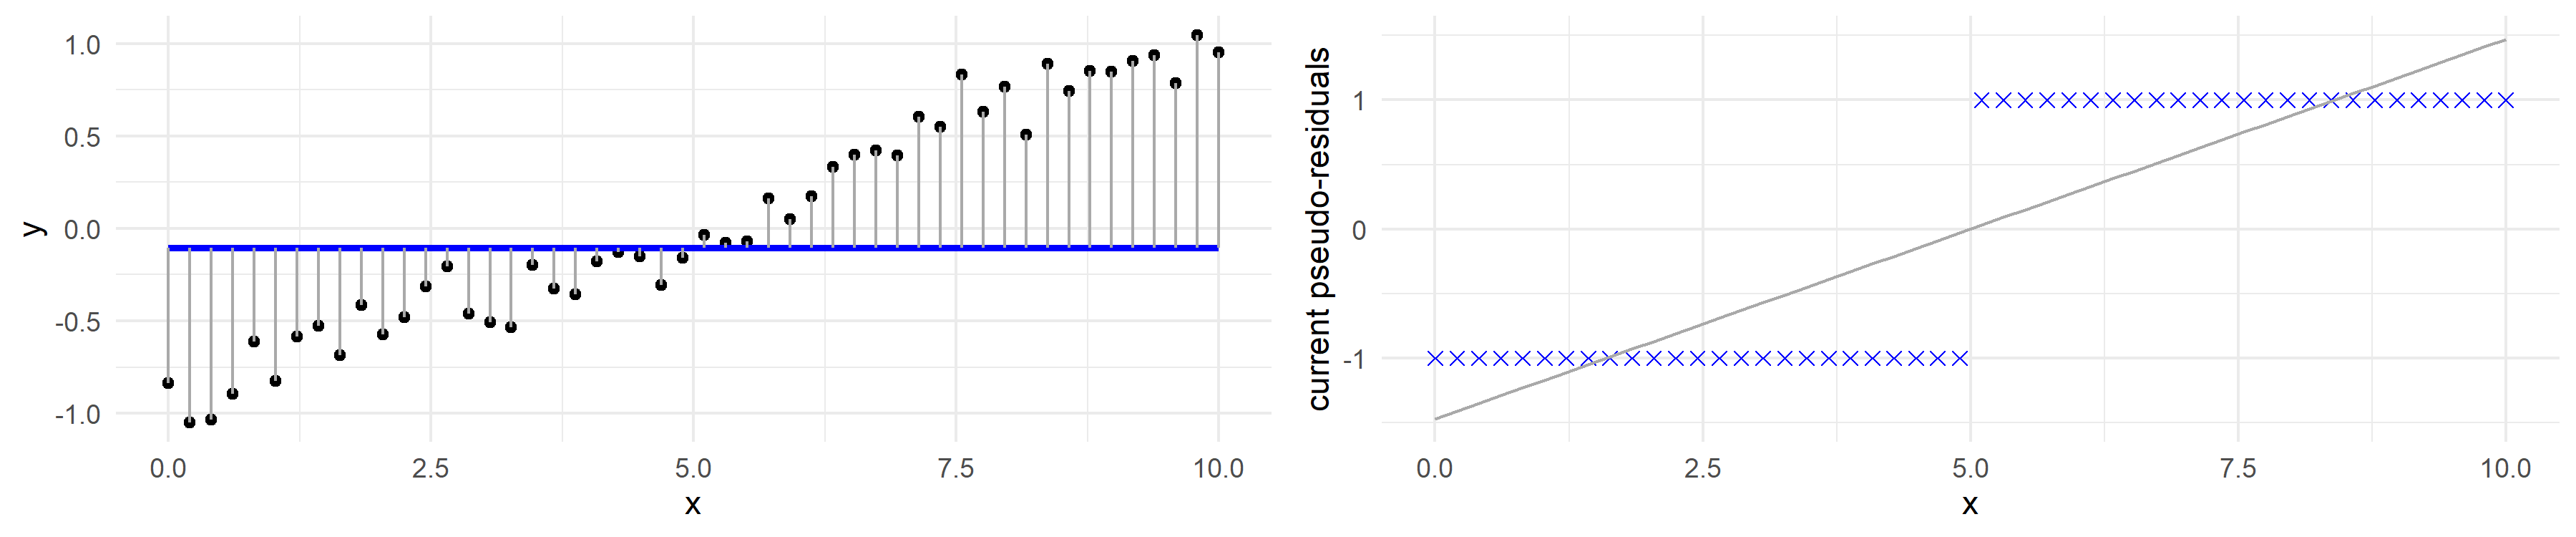
\includegraphics[width=\textwidth]{figure/illustration_gaussian_L1_lin_1.png}

\vfill
Iteration 1
}

% \only<2>{ 
% 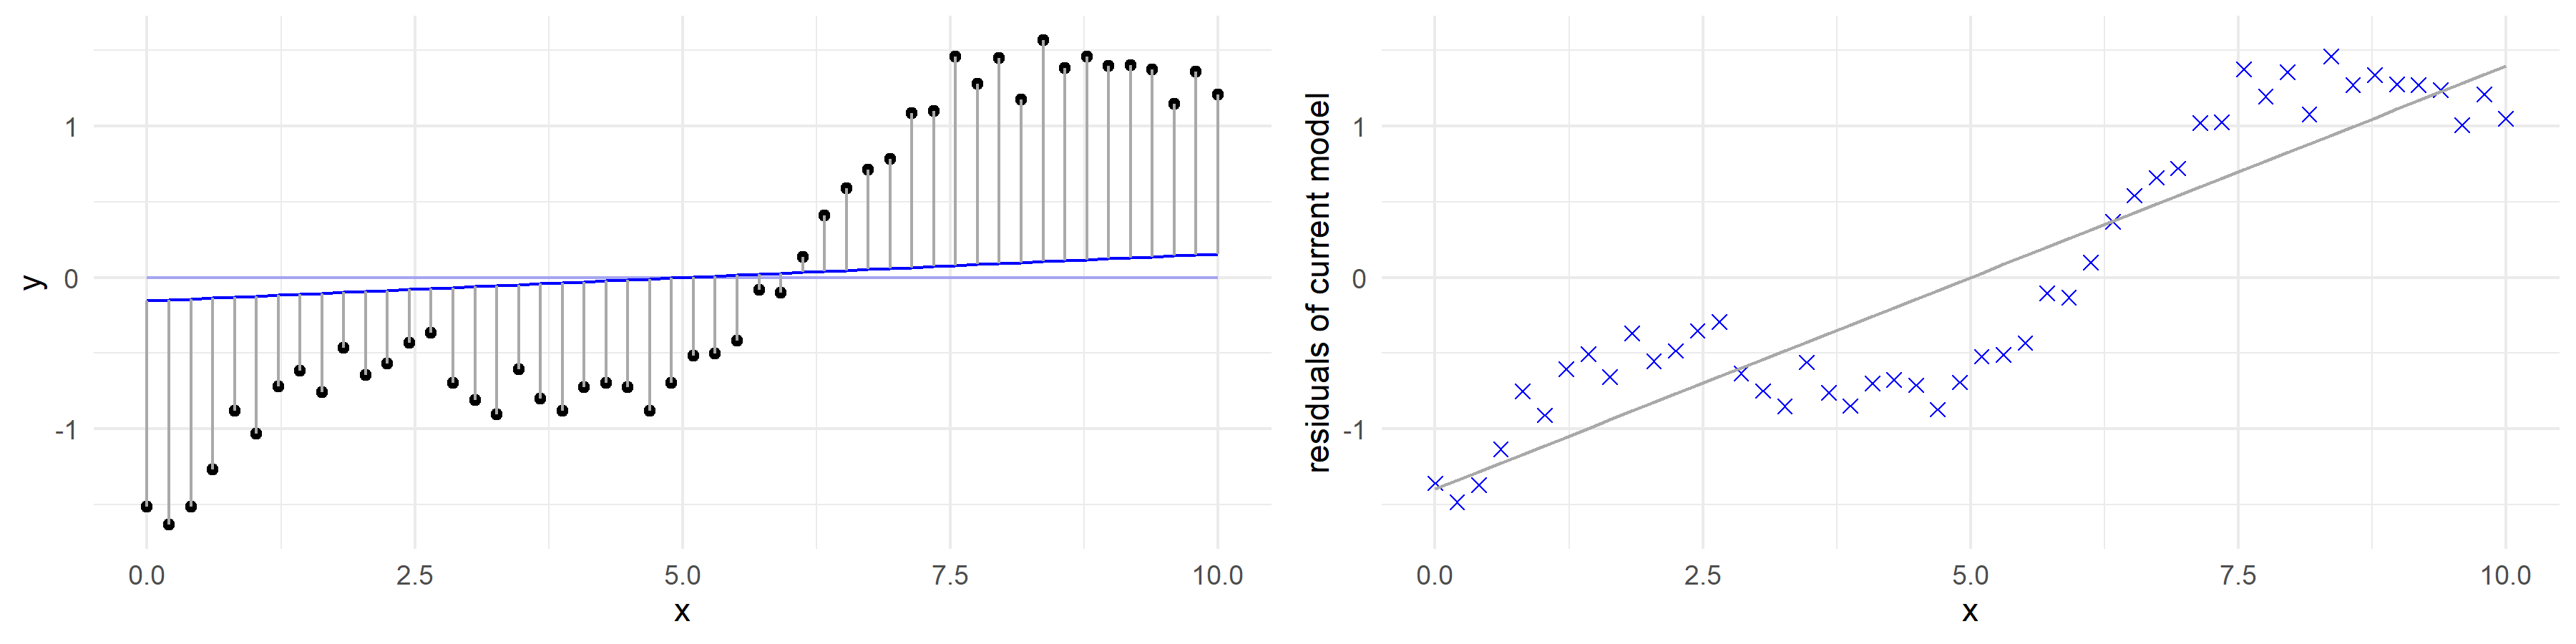
\includegraphics[width=\textwidth]{figure/illustration_gaussian_L2_lin_2.png}
% 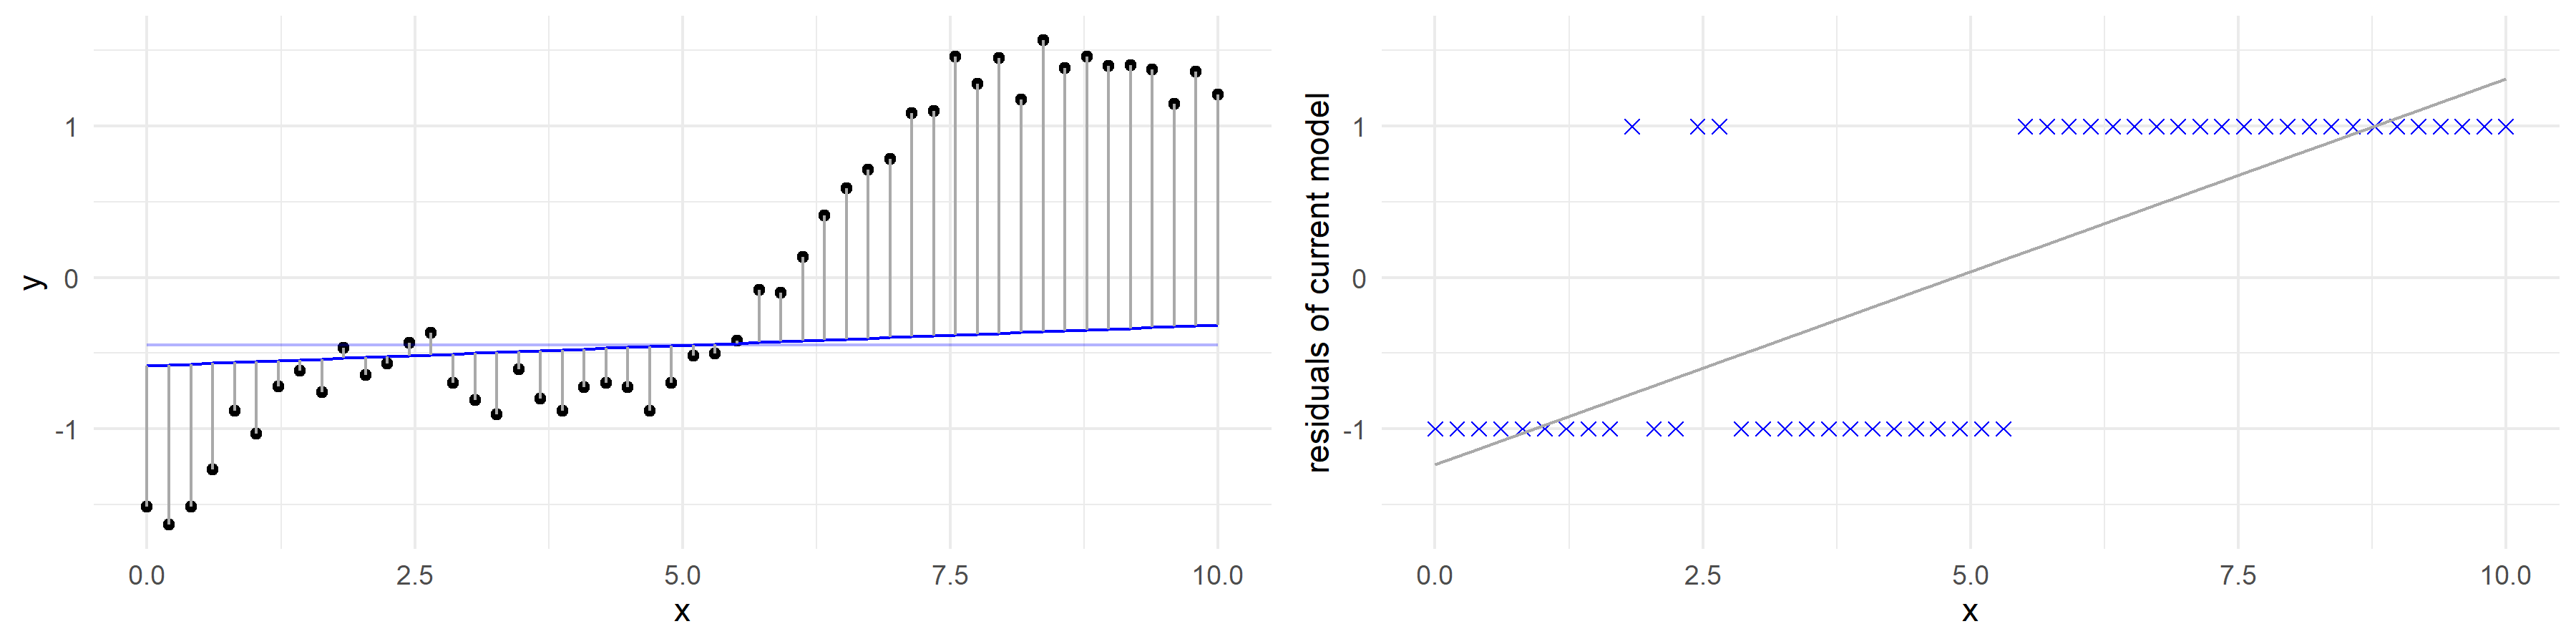
\includegraphics[width=\textwidth]{figure/illustration_gaussian_L1_lin_2.png}
% 
% \vfill
% Iteration 2
% }
% \only<3>{
% 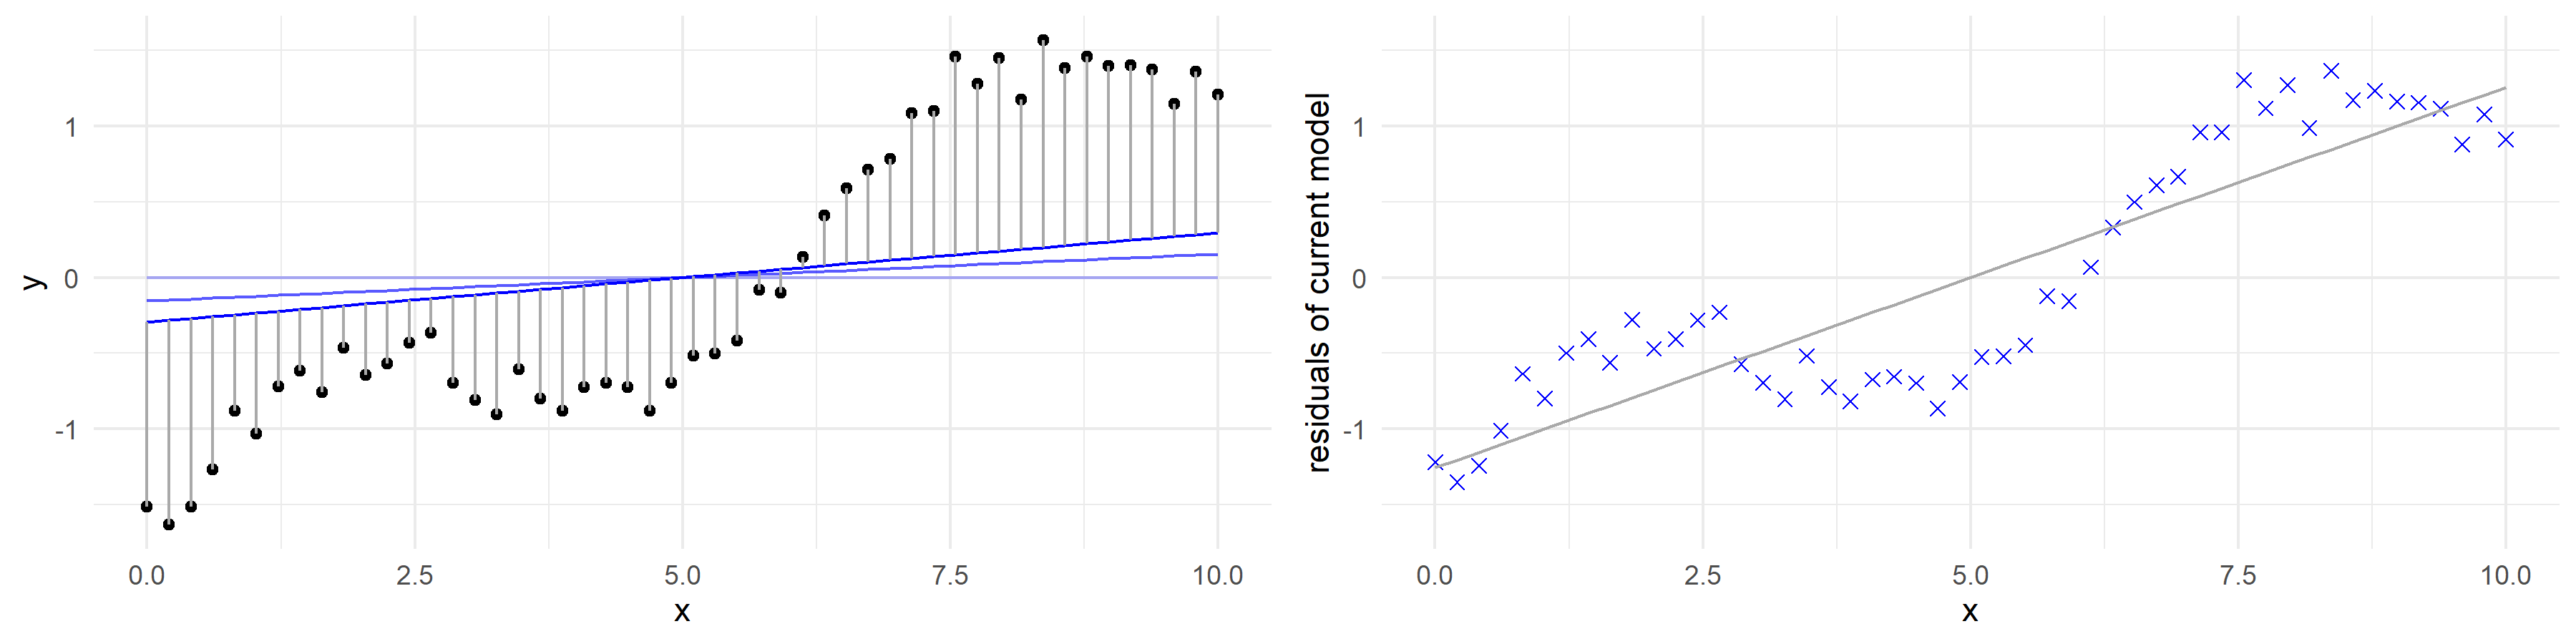
\includegraphics[width=\textwidth]{figure/illustration_gaussian_L2_lin_3.png}
% 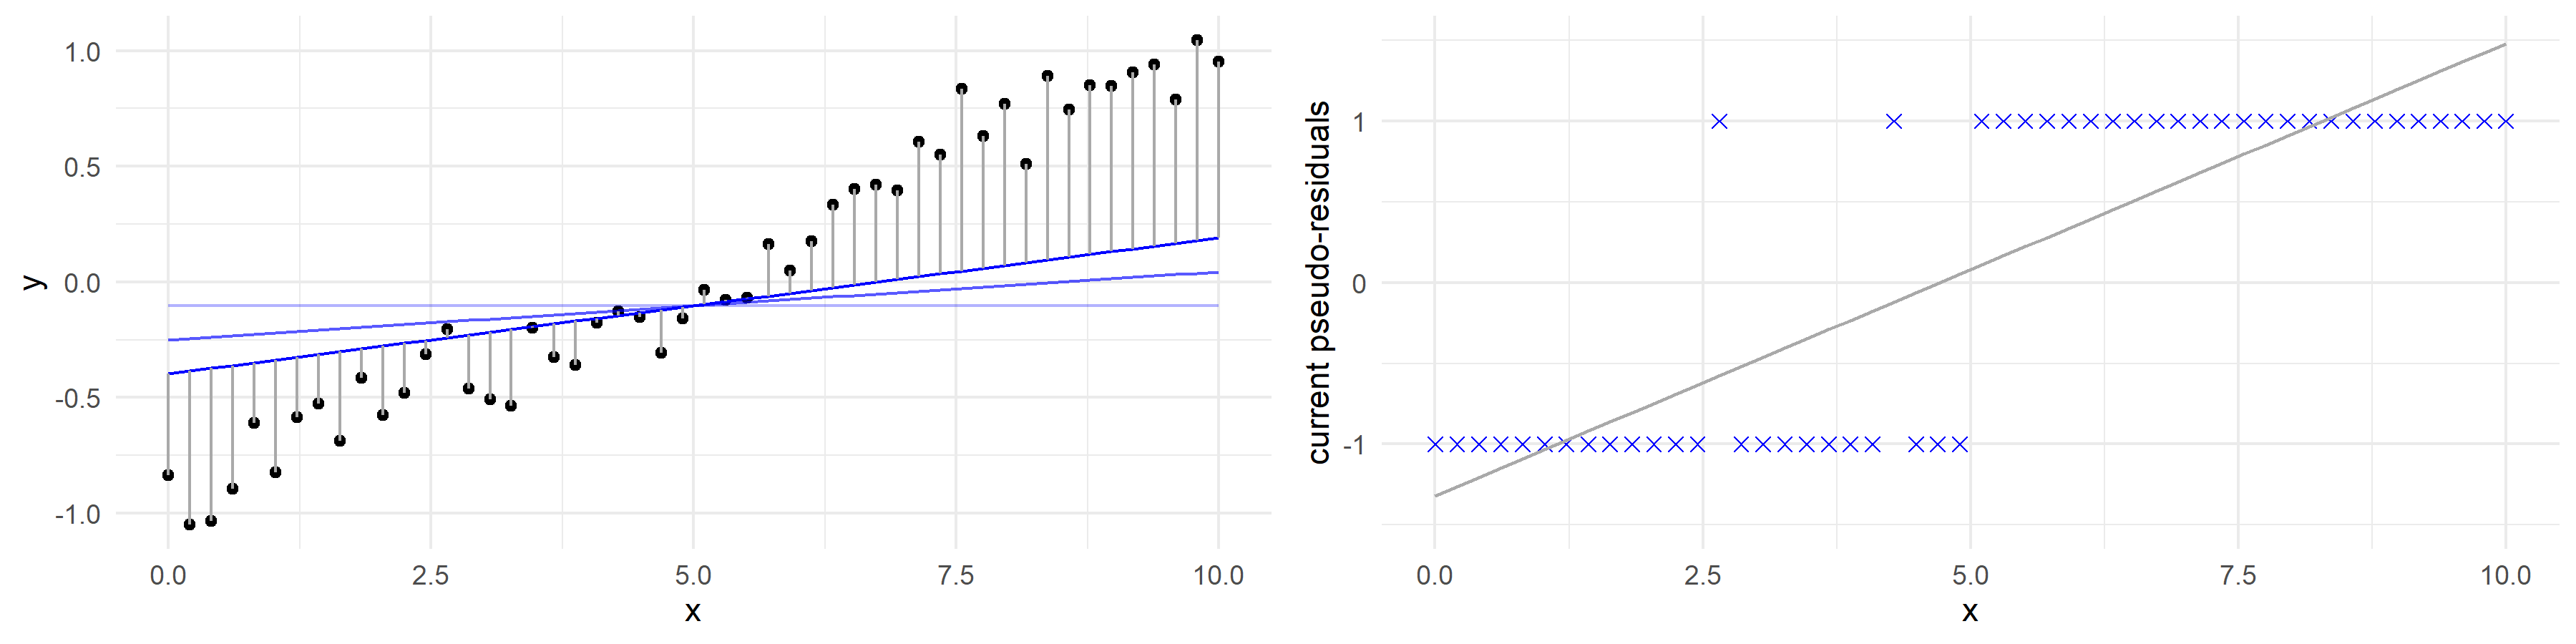
\includegraphics[width=\textwidth]{figure/illustration_gaussian_L1_lin_3.png}
% 
% \vfill
% Iteration 3
% }

\only<2>{
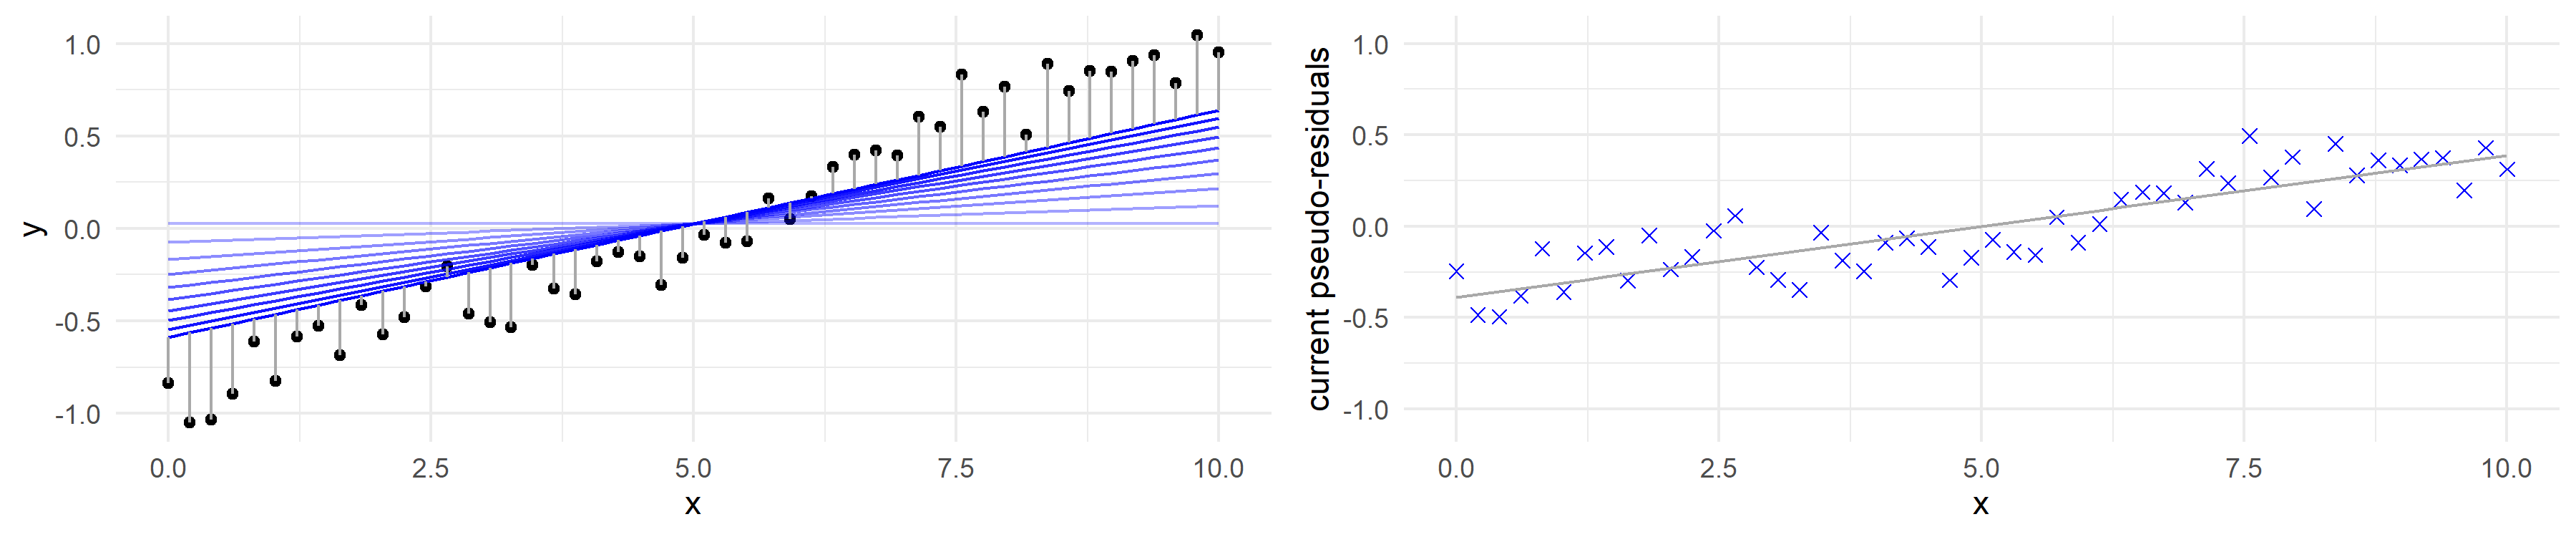
\includegraphics[width=\textwidth]{figure/illustration_gaussian_L2_lin_10.png}
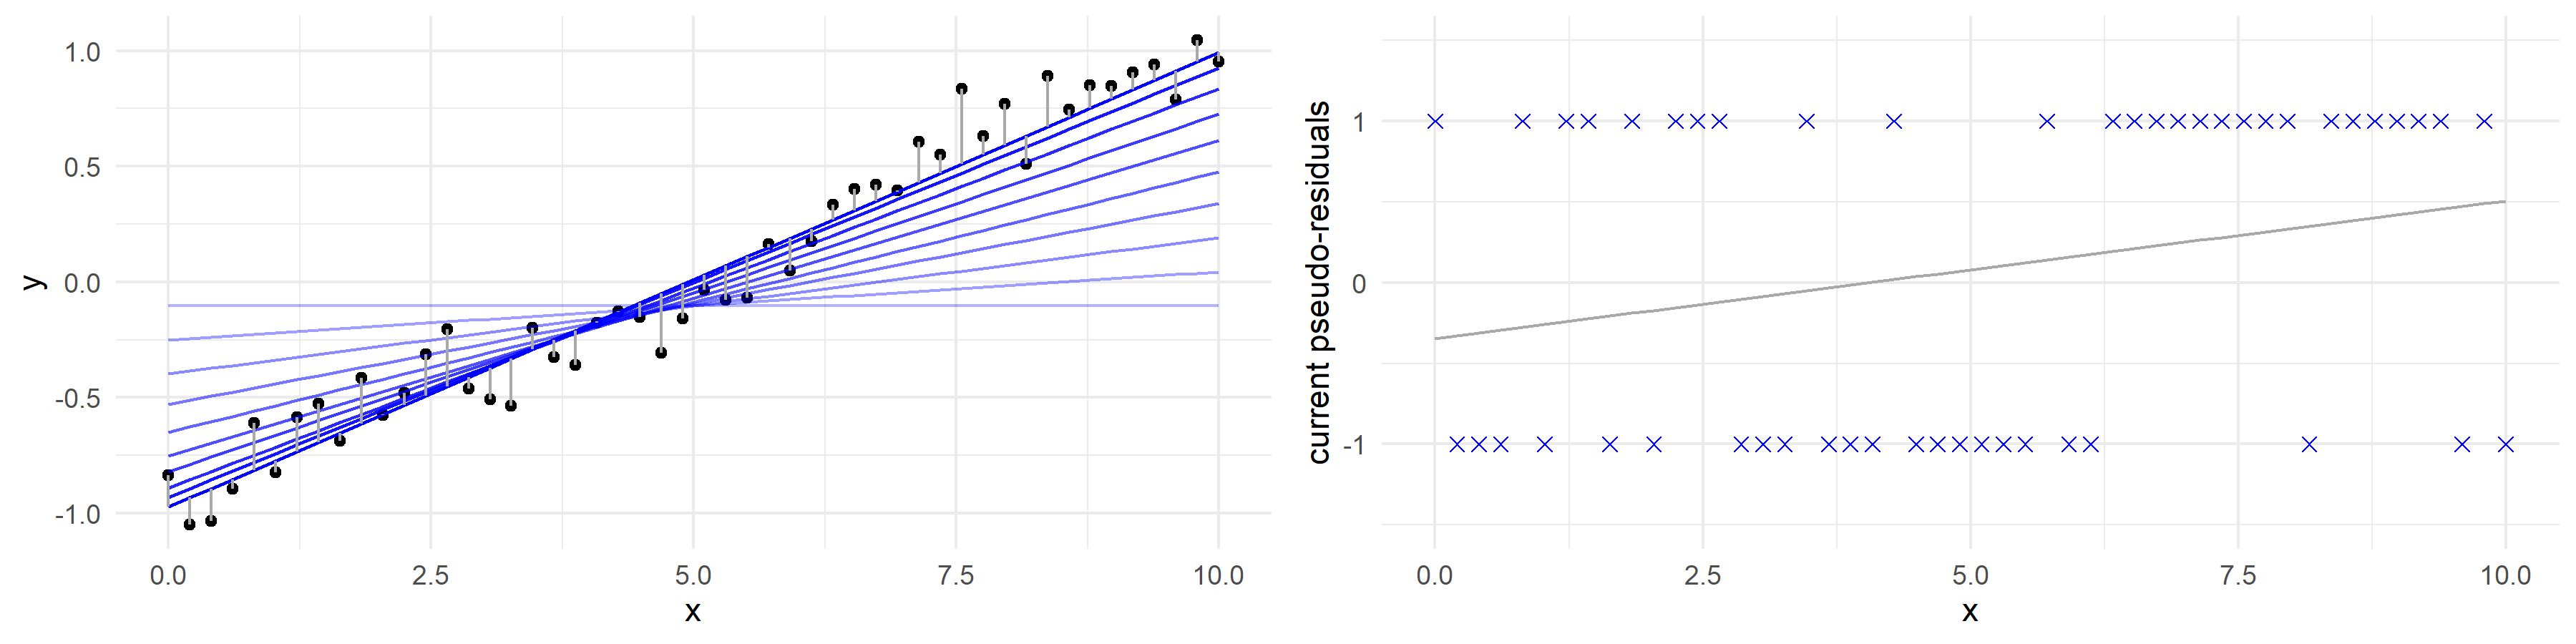
\includegraphics[width=\textwidth]{figure/illustration_gaussian_L1_lin_10.png}

\vfill
Iteration 10
}

\only<3>{ 
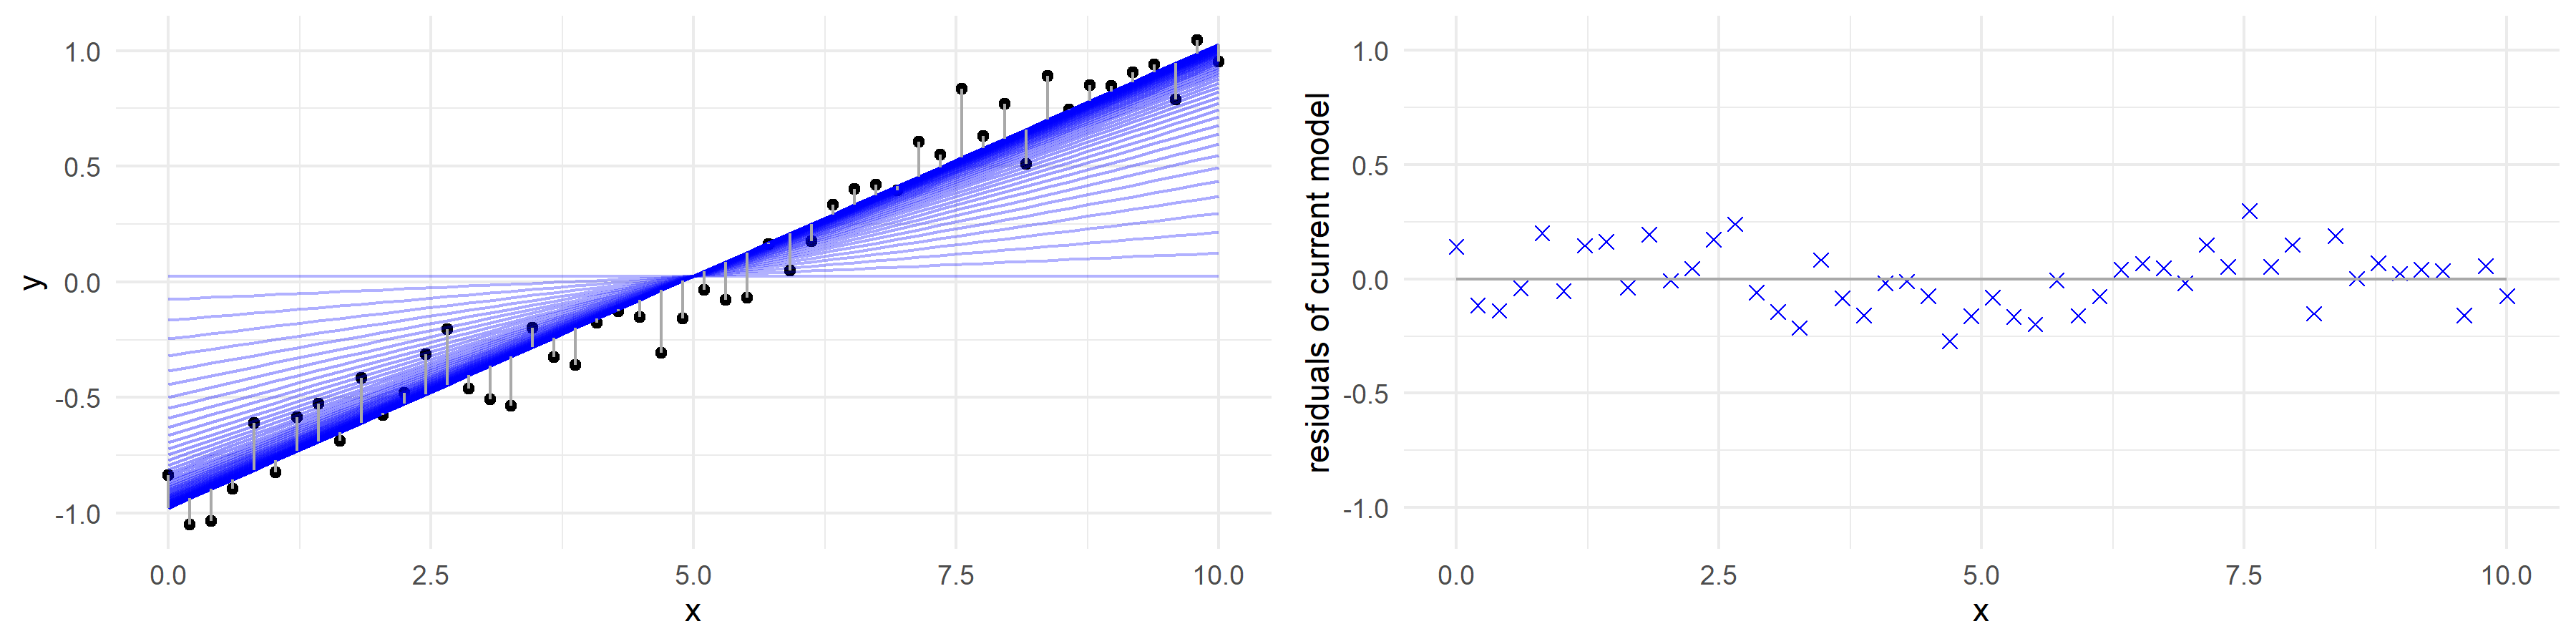
\includegraphics[width=\textwidth]{figure/illustration_gaussian_L2_lin_100.png}
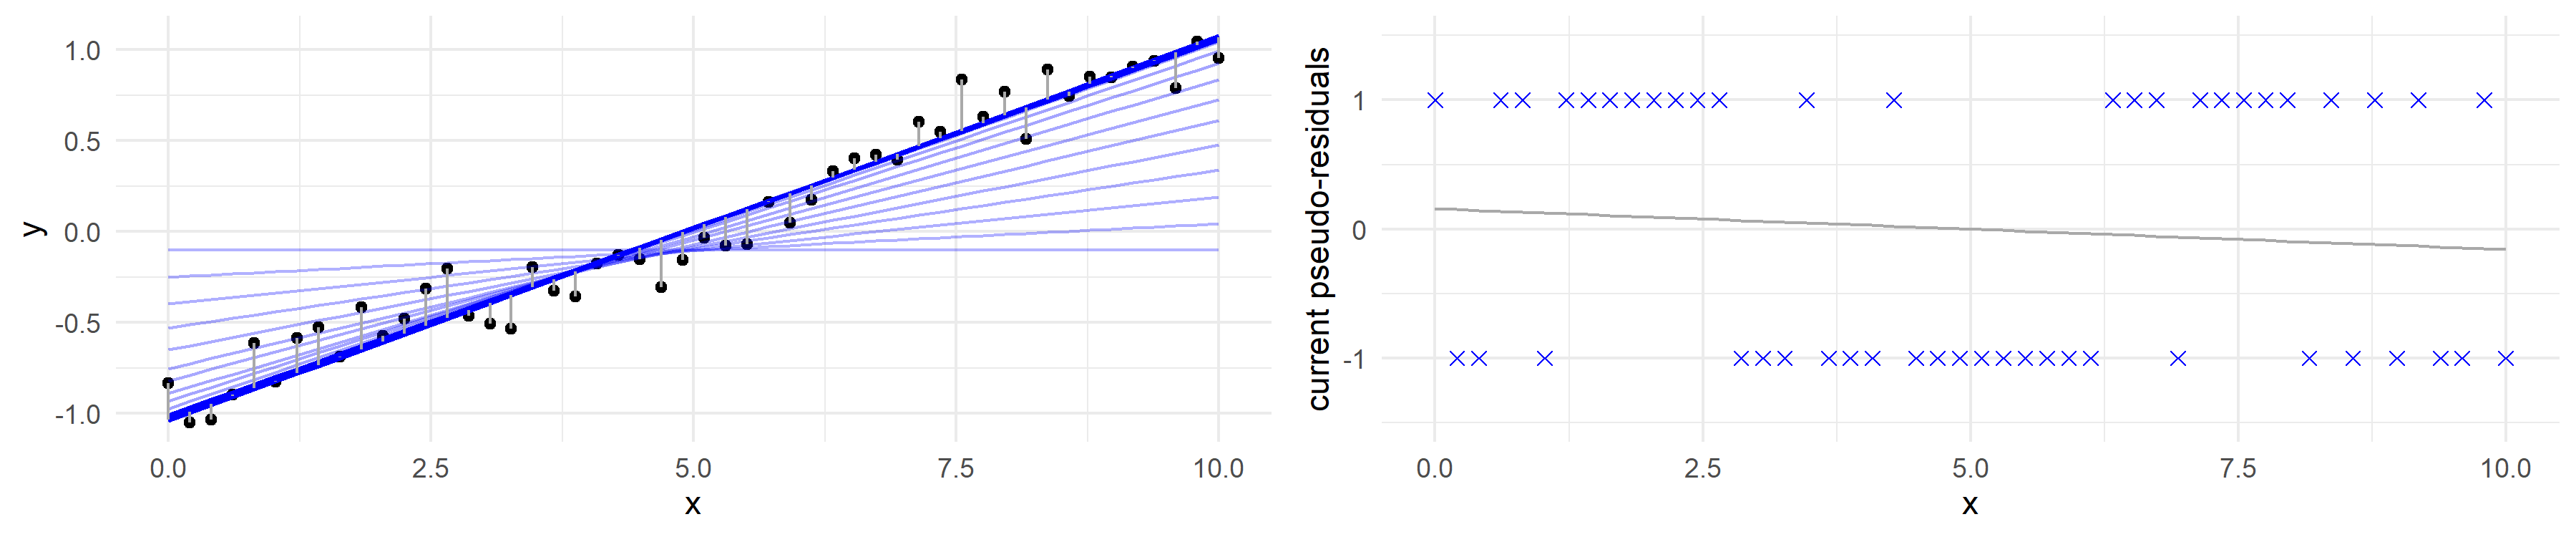
\includegraphics[width=\textwidth]{figure/illustration_gaussian_L1_lin_100.png}

\vfill
Iteration 100
}

\vfill

\footnotesize
For $L2$, as $\tilde r(f) = r(f)$, we find the optimal model in the very
first iteration; only the multiplicative learning rate slows down optimization.
In the $L1$ case the base learner LMs fit pseudo-residuals that differ from 
model residuals, leading to a less monotonic optimization path.

\end{frame}
% 
% \textbf{Iteration 1:} Step 1 to 3
% \begin{figure}
%   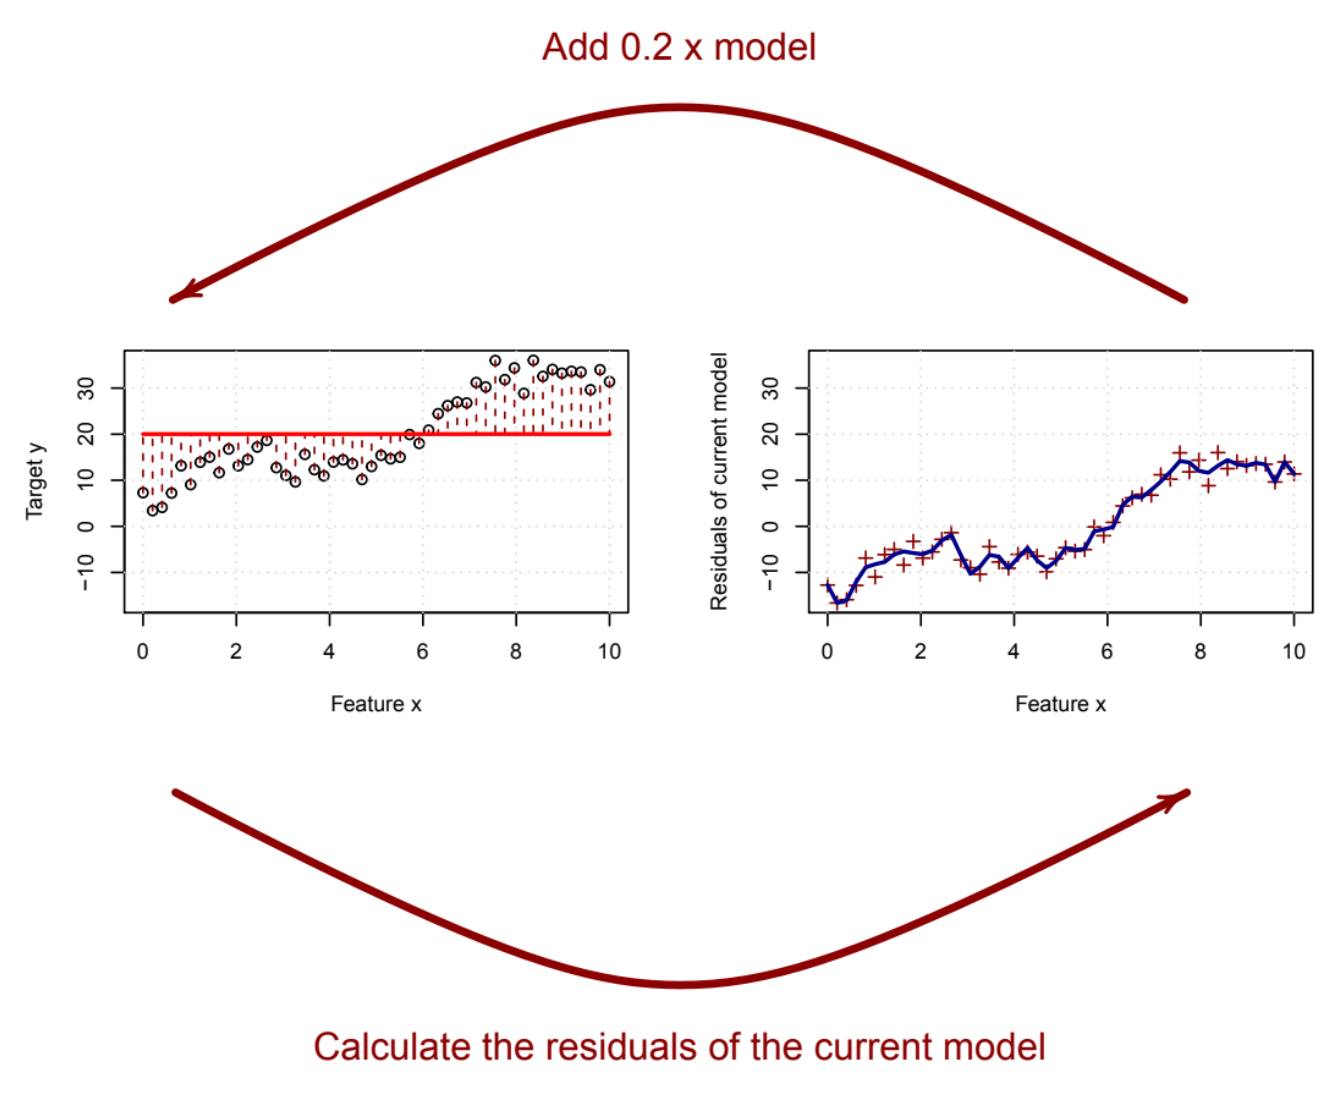
\includegraphics[width=0.7\textwidth]{figure_man/illustration2.png}
% \end{figure}
% 
% 
% \framebreak
% \textbf{Iteration 2:} Repeat Step 2 and 3
% \begin{figure}
%   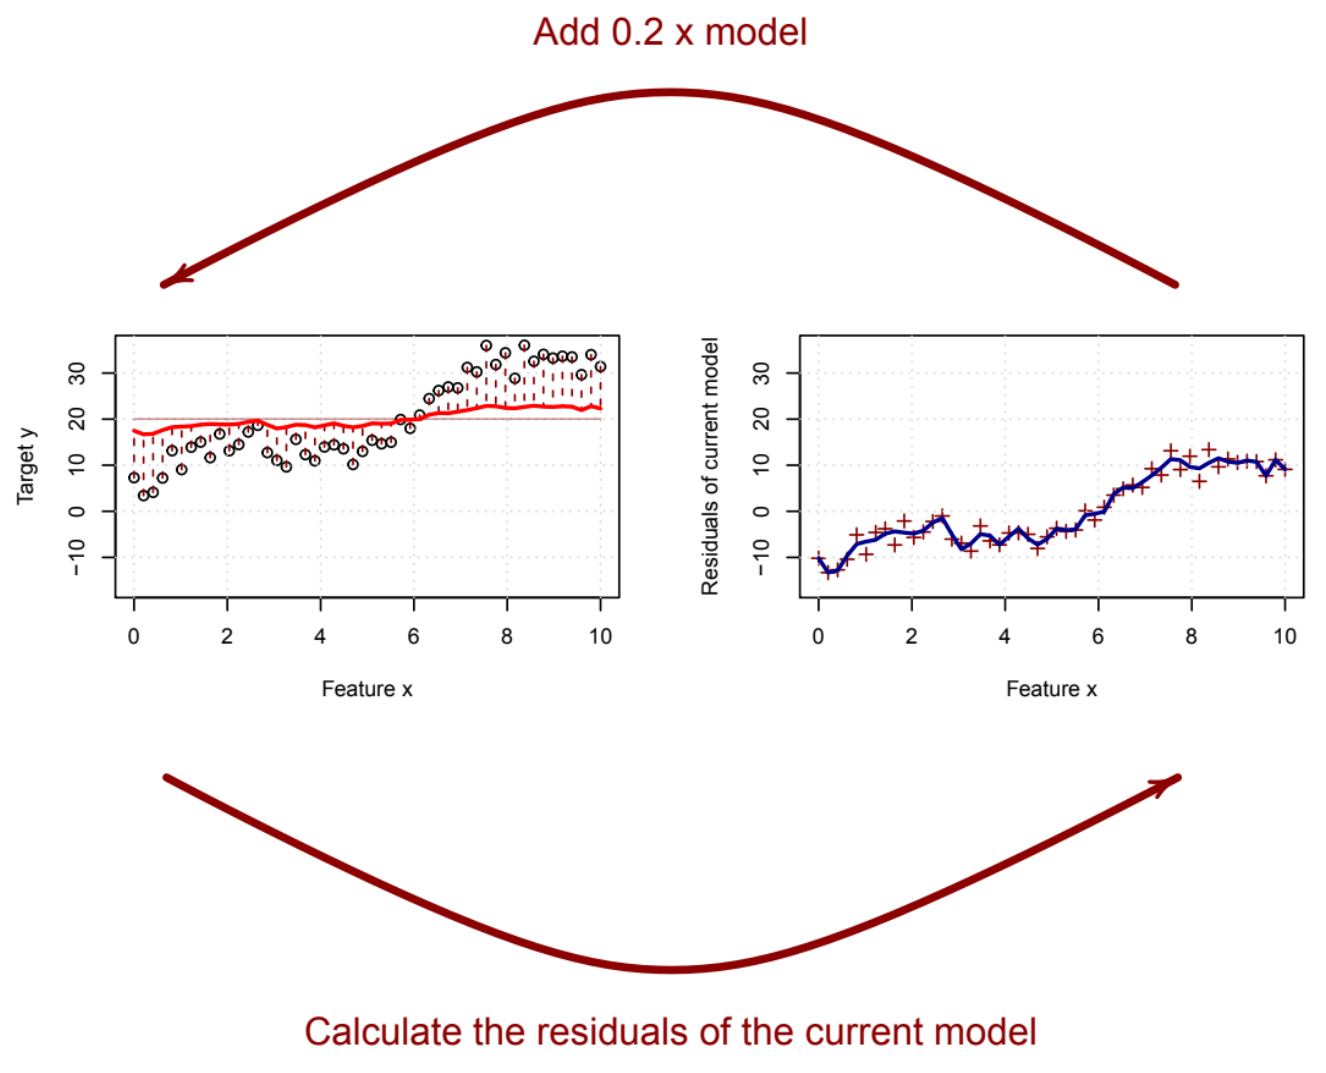
\includegraphics[width=0.7\textwidth]{figure_man/illustration3.png}
% \end{figure}
% 
% 
% \framebreak
% \textbf{Iteration 3:} Repeat Step 2 and 3
% \begin{figure}
%   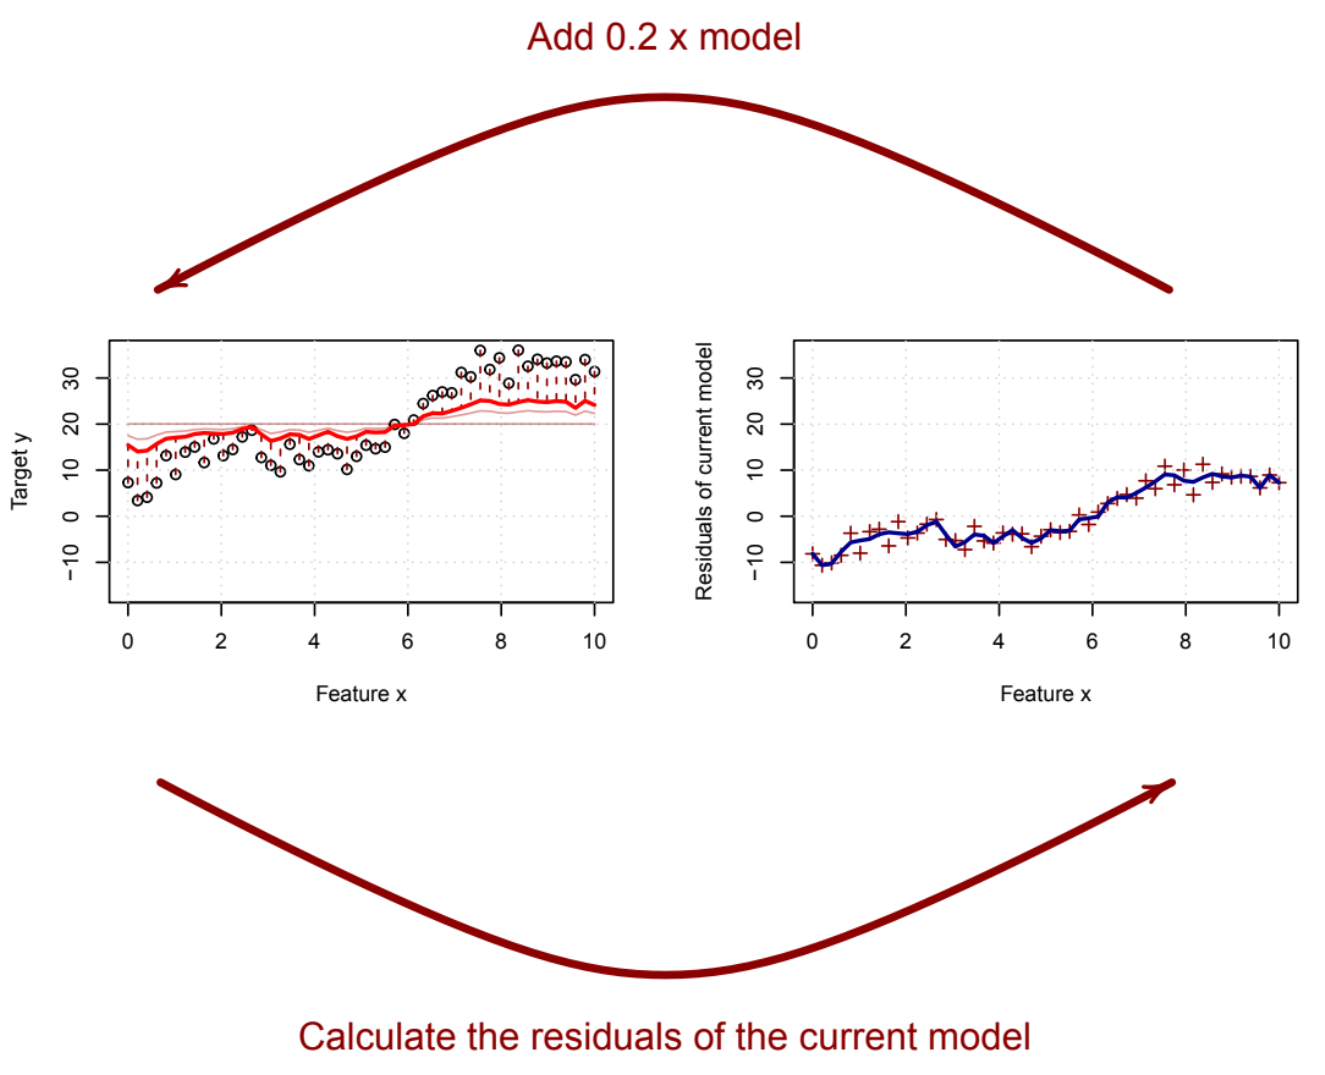
\includegraphics[width=0.7\textwidth]{figure_man/illustration4.png}
% \end{figure}
% 
% 
% \framebreak
% \textbf{Iteration 5:} Repeat Step 2 and 3
% \vspace{0.2cm}
% \begin{figure}
%   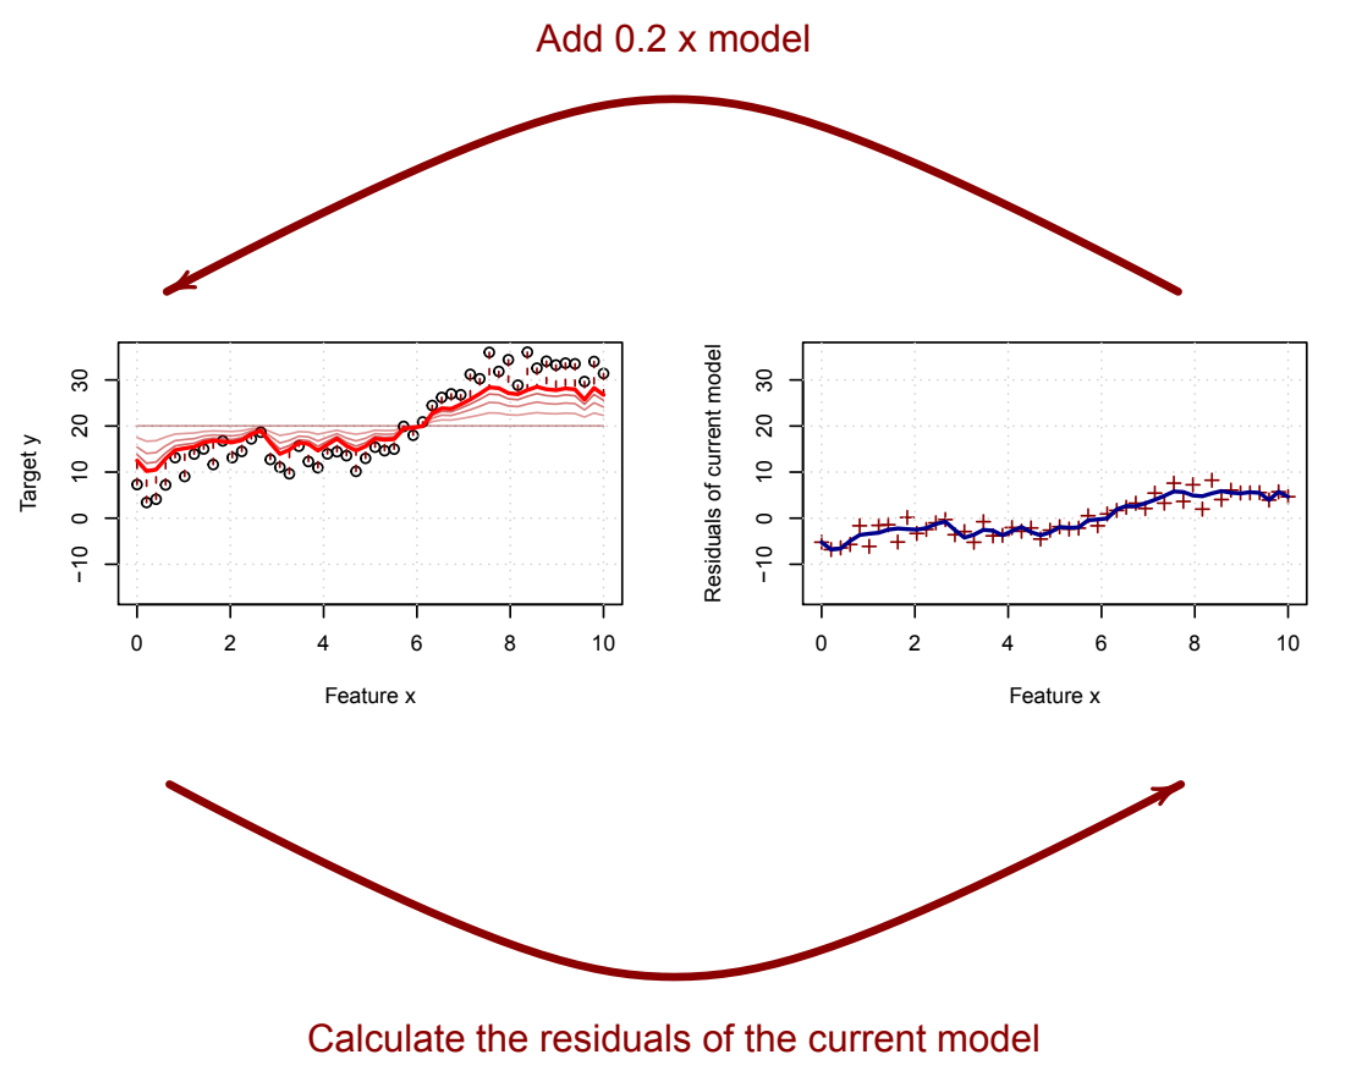
\includegraphics[width=0.7\textwidth]{figure_man/illustration5.png}
% \end{figure}
% 
% 
% \framebreak
% \textbf{Iteration 10:} Repeat Step 2 and 3
% \vspace{0.2cm}
% \begin{figure}
%   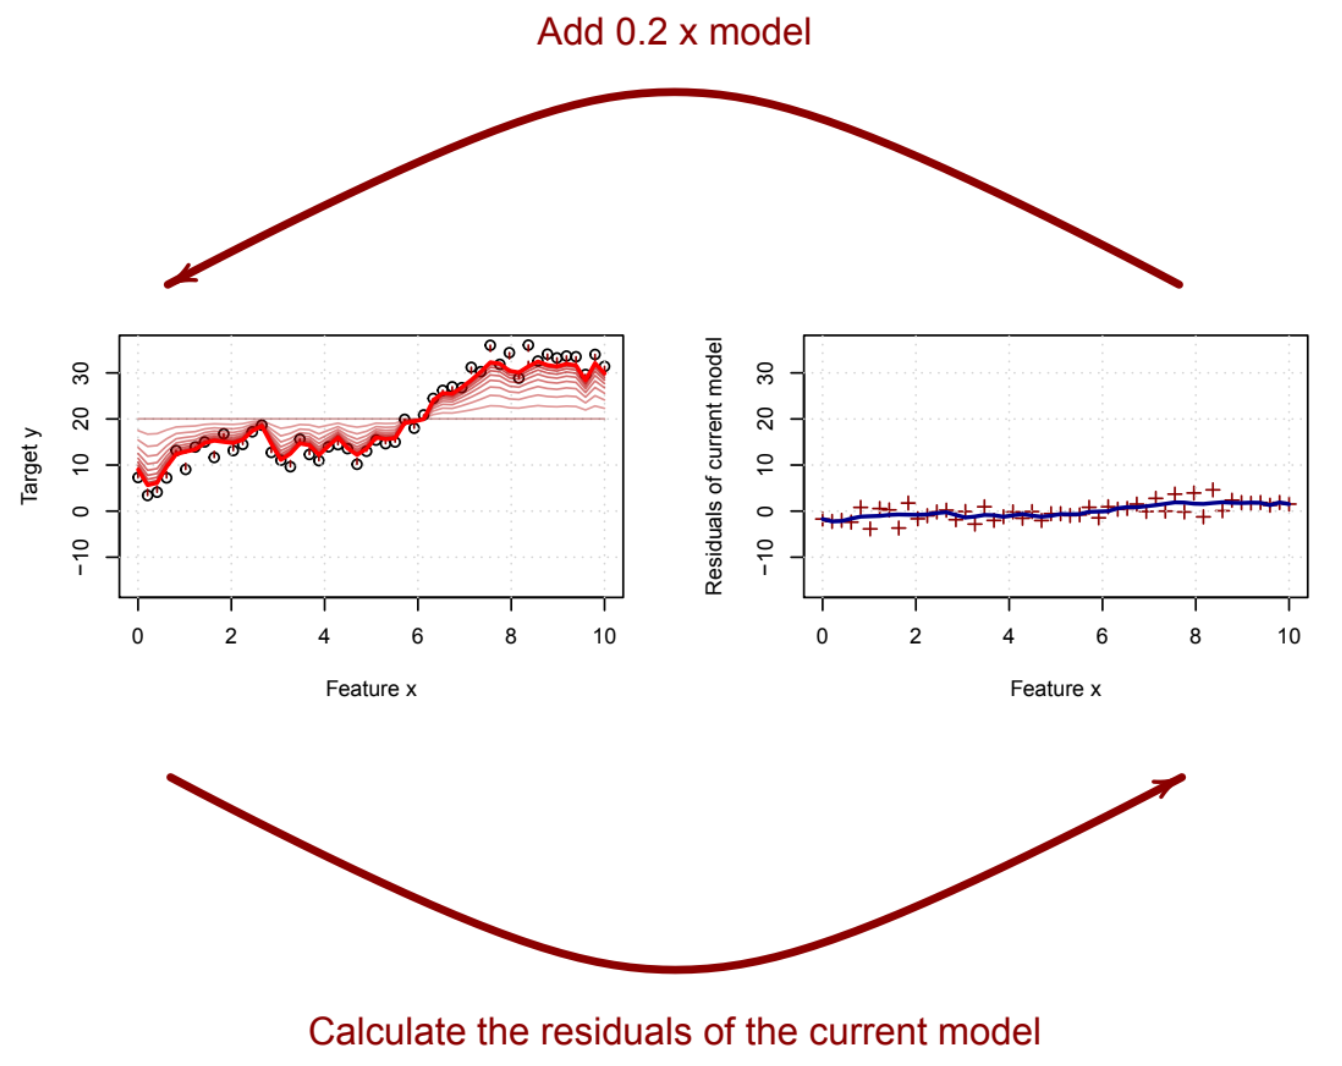
\includegraphics[width=0.7\textwidth]{figure_man/illustration6.png}
% \end{figure}
% 
% 
% \framebreak
% \textbf{Iteration 100:} Repeat Step 2 and 3
% \vspace{0.2cm}
% \begin{figure}
%   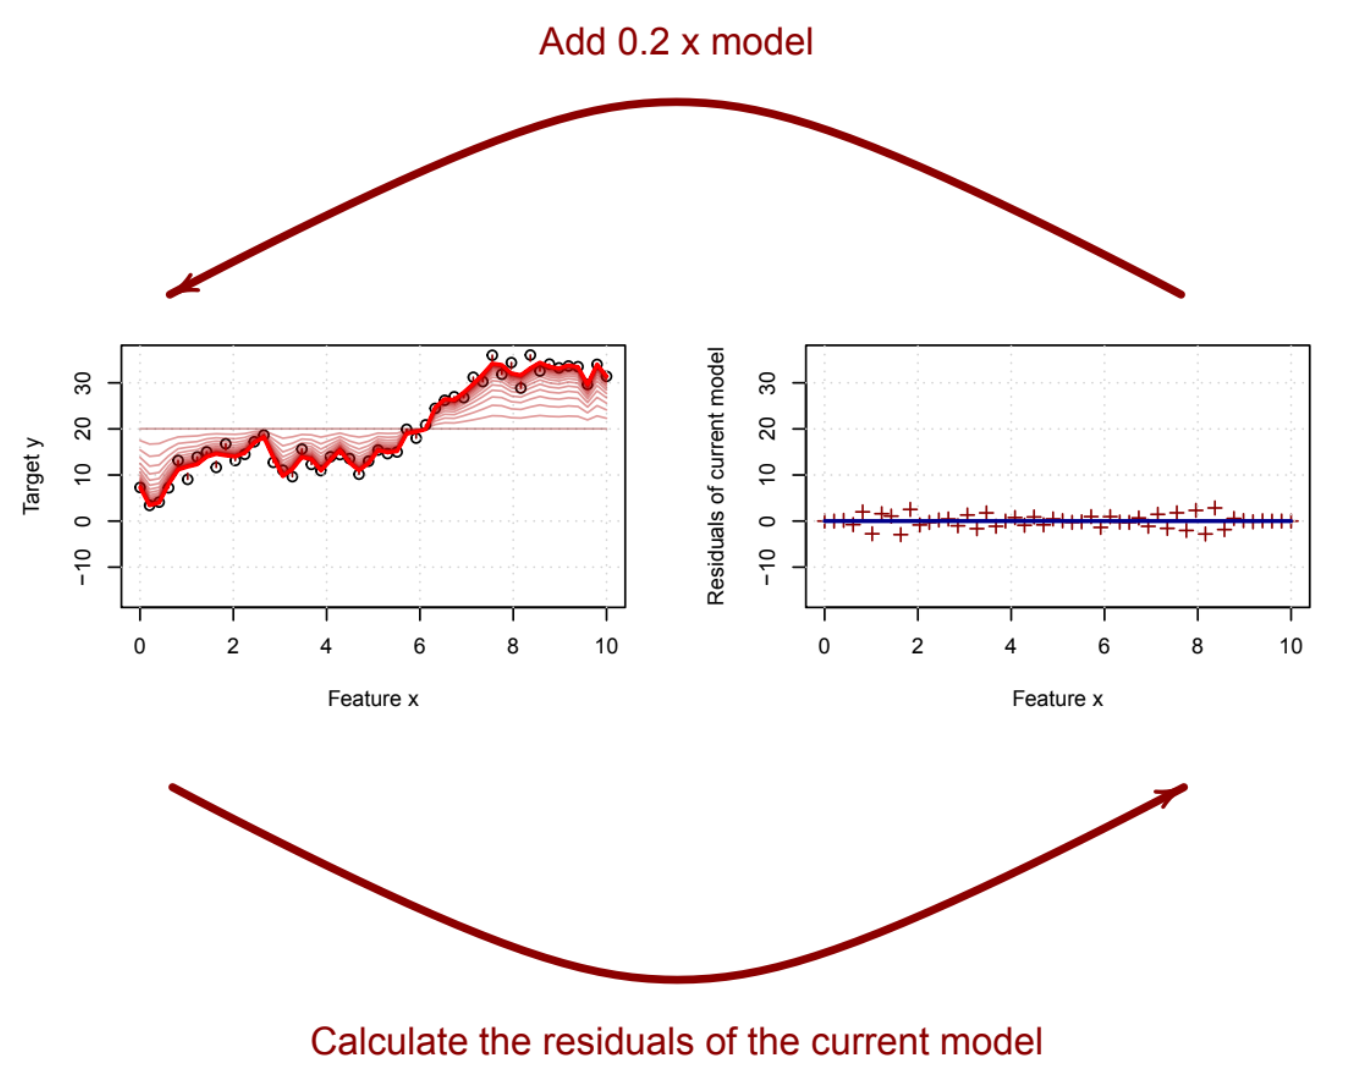
\includegraphics[width=0.7\textwidth]{figure_man/illustration7.png}
% \end{figure}
% 
% 
% \end{vbframe}

% ------------------------------------------------------------------------------

\begin{vbframe}{LM: gb vs gd}

\footnotesize

\begin{itemize}
  \item As we have seen, boosting with LMs and $L2$ 
  loss simply approaches the closed-form OLS solution with a speed determined by 
  the learning rate $\beta$.
  \item This is perfectly equivalent to fitting an LM via 
  \textbf{gradient descent}, as a gradient step in parameter space is a 
  gradient step in function space for this specific case.
  \item Recall the parameter update for GD with learning rate $\beta$:
  $\thetab^{[m+1]} \leftarrow \thetam - \beta \cdot \nabla_{\thetam} 
  \riske(\thetam) =  
  \thetam + \beta (-\Xmat^T \ydat + \Xmat^T\Xmat \thetam).$ \\
  \item Now compute the update for a boosted LM with current model 
  $\Xmat \thetam$ (note that adding a linear base learner to an LM is 
  equivalent to summing parameters):
  \begin{eqnarray*}
    \footnotesize
    \frac{\partial}{\partial \thetab^{[m+1]}} 
    \left \| (\ydat - \Xmat \thetam) - \Xmat \thetab^{[m+1]}) \right \|^2_2 
    &=& 0 \\
    -2\Xmat^T (\ydat - \Xmat \thetam) + 2\Xmat^T\Xmat 
    \thetab^{[m+1]} &=& 0 \\
    \thetab^{[m+1]} &=& (\Xmat^T\Xmat)^{-1} \Xmat^T 
    (\ydat - \Xmat \thetam) \\
    \thetab^{[m+1]} &=& (\Xmat^T\Xmat)^{-1} \Xmat^T \ydat
    - (\Xmat^T\Xmat)^{-1} \Xmat^T \Xmat \thetam \\
    \thetab^{[m+1]} &=& (\Xmat^T\Xmat)^{-1} \Xmat^T \ydat
    - \thetam % \quad \quad \textcolor{gray}{\rvert \cdot (-\Xmat^T\Xmat)} 
    \\
    \thetab^{[m+1]} &=& - \Xmat^T \ydat + \Xmat^T\Xmat 
    \thetam.
  \end{eqnarray*}
  $\Rightarrow \fh^{[m+1]} = \Xmat \tilde \thetab^{[m+1]} = 
  \Xmat \left( \thetam + \beta (-\Xmat^T \ydat + 
  \Xmat^T\Xmat \thetam) \right).$
\end{itemize}



\end{vbframe}

% ------------------------------------------------------------------------------

\endlecture
\end{document}

